\documentclass[12pt,a4paper]{report}

\usepackage[utf8]{inputenc}
\usepackage[T1]{fontenc}
\usepackage[italian,english]{babel}
\usepackage[a4paper,margin=2.6cm]{geometry}
\usepackage{graphicx}
\usepackage{booktabs}
\usepackage{array}
\usepackage{longtable}
\usepackage{multirow}
\usepackage{float}
\usepackage{enumitem}
\usepackage{hyperref}
\usepackage{xcolor}
\usepackage{listings}
\usepackage{caption}
\usepackage{float}

\hypersetup{
    colorlinks=true,
    linkcolor=blue,
    urlcolor=blue,
    pdftitle={Relazione progetto Base di Dati - Zoo Manager}
}

\lstdefinestyle{sqlstyle}{
    language=SQL,
    basicstyle=\ttfamily\small,
    keywordstyle=\bfseries\color{blue!70!black},
    commentstyle=\itshape\color{gray!70!black},
    stringstyle=\color{orange!70!black},
    showstringspaces=false,
    breaklines=true,
    frame=single,
    columns=fullflexible
}

\newcommand{\screenshotplaceholder}[2]{
\begin{figure}[H]
\centering
\fbox{\begin{minipage}[c][0.23\textheight][c]{0.86\textwidth}
\centering
\textbf{#1}\\[6pt]
#2
\end{minipage}}
\caption{#1}
\end{figure}
}

\newcolumntype{L}[1]{>{\raggedright\arraybackslash}p{#1}}
\newcolumntype{C}[1]{>{\centering\arraybackslash}p{#1}}

\begin{document}

\begin{titlepage}
\centering
\vspace*{2cm}
{\Large Relazione\par}

\vspace{0.4cm}
\vspace{1.5cm}
{\large Progetto di base di dati per il gestionale di uno zoo\par}
\vspace{1.5cm}
\hfill
\begin{minipage}{0.4\textwidth}
    \small
    Francesco Caravita – 0001161188 \newline
    francesco.caravita2@studio.unibo.it 
    \newline
    Luca Mularoni – 0001162772 \newline
    luca.mularoni@studio.unibo.it
\end{minipage}
\vfill

\end{titlepage}

\tableofcontents
\clearpage

\iffalse % INIZIO COMMENTO 
\chapter{Introduzione}

Il progetto realizza il sistema informativo di supporto a uno zoo, con l'obiettivo di
gestire in modo integrato sia i dati amministrativi sia quelli operativi.
Il database è progettato per conservare le informazioni sugli animali, sulle specie,
sugli habitat, sulle aree e sui recinti, ma anche sul personale, sui turni di lavoro,
sulle visite mediche, sugli ordini di cibo, sulla biglietteria e sulle transazioni
economiche.

La soluzione è stata pensata come un applicativo gestionale interno, accessibile
attraverso un'interfaccia JavaFX, che dialoga con un database PostgreSQL tramite
DAO JDBC. L'applicazione è organizzata secondo una logica MVC: le \emph{view}
gestiscono l'interfaccia grafica, i \emph{controller} governano le operazioni e i
\emph{DAO} incapsulano l'accesso ai dati.

\section{Obiettivi del sistema}

Il sistema deve permettere:

\begin{itemize}[itemsep=2pt]
    \item la gestione dell'anagrafica degli animali;
    \item la classificazione delle specie in base a stato di conservazione, habitat e famiglia;
    \item la gestione delle aree e dei recinti;
    \item la pianificazione dei turni del personale;
    \item la registrazione delle visite mediche;
    \item la gestione della biglietteria e delle transazioni;
    \item la registrazione degli ordini giornalieri di cibo e dei fornitori;
    \item il controllo di saldo, statistiche e dati di supporto alle decisioni.
\end{itemize}

\fi % FINE COMMENTO


\chapter{Analisi dei requisiti}

\section{Definizione delle specifiche in linguaggio naturale ed estrazione dei concetti principali}

Si vuole realizzare un sistema informativo per la gestione di uno zoo, che permetta di organizzare, l’archivio degli animali, le attività interne, monitorare la situazione economica e gestire la vendita dei biglietti ai visitatori. 

Lo zoo ospita numerosi animali di cui gestisce ogni aspetto, dalla pianificazione della dieta fino al monitoraggio dello stato di salute attraverso visite e trattamenti medici. Per ciascun animale il sistema memorizza informazioni anagrafiche quali nome, specie di appartenenza, età, sesso e stato di salute corrente. Ogni animale viene assegnato a un recinto specifico, che condivide con altri esemplari della medesima specie. I recinti sono identificati da un codice univoco e descritti da una tipologia (ad esempio acquatico, terrestre o tropicale), da una capienza massima da rispettare e dall'area dello zoo in cui sono collocati. Un recinto può ospitare più animali contemporaneamente, a condizione che non venga superata la capienza stabilita. 

Per quanto riguarda la gestione del personale, si vogliono memorizzare i dati anagrafici dei dipendenti, il ruolo svolto (ad esempio veterinario, custode, guida) e i contatti. I dipendenti vengono assegnati a turni di lavoro organizzati su base giornaliera o settimanale; per ogni turno si registrano il dipendente assegnato, l’orario di inizio e fine e l’area dello zoo in cui presta servizio. Un dipendente può avere più turni, ma non può essere assegnato a più turni contemporaneamente nello stesso intervallo orario. 

Lo zoo offre ai visitatori diverse tipologie di biglietto, tra cui biglietto standard, ridotto e speciale (ad esempio comprensivo di visita guidata). Per ogni tipologia si vogliono memorizzare prezzo e descrizione, mantenendo eventualmente uno storico delle variazioni di prezzo nel tempo. 

I visitatori possono acquistare uno o più biglietti tramite una singola prenotazione. Per ogni acquisto si registrano la data, la quantità di biglietti, la tipologia scelta e il prezzo totale. Nel caso di acquisti di gruppo, più biglietti possono essere associati alla stessa prenotazione. Il sistema consente di mantenere uno storico completo delle vendite, utile per analisi e statistiche. 

Per quanto riguarda la gestione economica, il sistema tiene traccia anche delle spese dello zoo. Ogni spesa è caratterizzata da una data, un importo, una categoria (ad esempio alimentazione animali, manutenzione strutture, altre spese operative) e una descrizione opzionale. Questo permette di confrontare le entrate derivanti dalla vendita dei biglietti con le uscite sostenute. 

Il sistema deve consentire di registrare e aggiornare le informazioni relative ad animali, recinti, personale, turni di lavoro, vendite e spese. Inoltre, deve permettere la consultazione dello storico dei dati e la produzione di statistiche, come il numero di biglietti venduti in un certo periodo, il ricavo totale, il confronto tra entrate e uscite, i periodi di maggiore affluenza, i dipendenti con più turni assegnati e i recinti con il maggior numero di animali. 

Infine, alcune operazioni sono riservate all’amministratore del sistema, che può gestire le specie animali, creare o eliminare recinti e aree, inserire e modificare i dati dei dipendenti, pianificare i turni di lavoro, definire le tipologie di biglietto e i relativi prezzi, nonché registrare e controllare le spese e accedere a tutte le statistiche globali del sistema. 

\subsection*{Concetti principali estratti}

I concetti centrali del dominio sono:
\begin{itemize}[itemsep=2pt]
    \item \textbf{Animale}, \textbf{Specie}, \textbf{Habitat}, \textbf{Famiglia specie}, \textbf{Stato esistenza};
    \item \textbf{Area}, \textbf{Recinto}, \textbf{Tipo area}, \textbf{Tipo recinto};
    \item \textbf{Dipendente}, \textbf{Mansione}, \textbf{Turno}, \textbf{Stipendio storico};
    \item \textbf{Visita medica};
    \item \textbf{Utente} con ruoli di accesso;
    \item \textbf{Tipo biglietto}, \textbf{Scontrino}, \textbf{Dettaglio scontrino}, \textbf{Transazione}, \textbf{Categoria transazione};
    \item \textbf{Fornitore}, \textbf{Tipo cibo}, \textbf{Fornitore cibo}, \textbf{Ordine giornaliero}.
\end{itemize}


\iffalse % INIZIO COMMENTO 
\fi % FINE COMMENTO
\section{Intervista}


Di seguito è riportata una sintesi dell'intervista svolta, da cui
sono emersi i requisiti fondamentali del sistema.

\begin{longtable}{L{4cm} L{10cm}}
\toprule
\textbf{Domanda} & \textbf{Risposta / indicazione del committente} \\
\midrule
\endhead
Quali categorie di utenti devono usare il sistema? &
Il sistema è usato dal personale dello zoo con ruoli diversi: amministratore, cassiere, guardiano e veterinario. Alcune sezioni sono accessibili anche in consultazione da parte degli utenti pubblici. \\

Quali dati devono essere memorizzati? &
Devono essere memorizzati animali, specie, habitat, famiglie tassonomiche, aree, recinti, dipendenti, turni, visite mediche, biglietti, scontrini, transazioni, ordini di cibo, fornitori e donazioni. \\

Quali operazioni devono essere più immediate? &
Le operazioni più frequenti sono la vendita dei biglietti, la consultazione del saldo, la gestione degli ordini di cibo, l'inserimento delle visite mediche e la visualizzazione dell'anagrafica degli animali. \\

Esistono vincoli importanti? &
Sì. Ogni animale appartiene a una sola specie, ogni recinto si trova in una sola area, ogni dipendente ha una mansione, ogni visita medica è svolta da un veterinario, e gli animali possono cambiare recinto nel tempo. \\

Serve tracciare la storia delle modifiche? &
Sì, per alcuni aspetti è essenziale: collocazione degli animali, stipendio dei dipendenti, visite mediche, turni e movimenti economici devono essere storicizzati. \\
\bottomrule
\end{longtable}

\section{Rilevamento delle ambiguità e correzioni proposte}

Dalla specifica iniziale emergono alcune ambiguità che sono state risolte in fase di progettazione.

\begin{longtable}{L{4.2cm} L{5cm} L{5.2cm}}
\toprule
\textbf{Elemento ambiguo} & \textbf{Problema} & \textbf{Correzione adottata} \\
\midrule
\endhead
\texttt{Utente} &
Può essere confuso con un visitatore finale. &
Nel database rappresenta un operatore autenticato del gestionale, associato a un dipendente e a un ruolo applicativo. \\

\texttt{Stato esistenza} &
Il nome può far pensare allo stato dell'animale. &
È usato per la classificazione della specie, ad esempio per indicare lo stato di conservazione secondo categorie come LC, VU, EN, CR. \\

\texttt{Transazione} e \texttt{Scontrino} &
Rischiano di apparire ridondanti. &
Lo scontrino rappresenta l'atto di vendita al cliente, mentre la transazione rappresenta il movimento contabile, che può essere di entrata o uscita. \\

\texttt{Vivo} e \texttt{Data uscita} &
Potrebbero sembrare informazioni sovrapposte. &
La coppia è mantenuta perché consente di distinguere tra animale presente, animale trasferito e animale deceduto, conservando la cronologia. \\

\texttt{Storico collocazione} &
Senza una storia dei recinti si perderebbe l'evoluzione degli spostamenti. &
Si introduce un'entità storica separata per registrare le permanenze nel tempo di ciascun animale nei recinti. \\

\texttt{Ordine giornaliero} &
Può sembrare un generico acquisto. &
È specializzato in ordini di cibo, collegato a fornitore, tipo di cibo e transazione economica associata. \\
\bottomrule
\end{longtable}



\chapter{Progettazione concettuale}

\section{Schema scheletro}

Lo schema scheletro contiene le entità principali del dominio:
\textbf{Animale}, \textbf{Specie}, \textbf{Area}, \textbf{Recinto}, \textbf{Dipendente},
\textbf{Visita medica}, \textbf{Utente}, \textbf{Tipo biglietto}, \textbf{Scontrino},
\textbf{Transazione}, \textbf{Fornitore}, \textbf{Ordine giornaliero}, \textbf{Donazione}.

In questa fase le entità sono state introdotte nella forma più immediata, con una
selezione minima di attributi e senza ancora esplicitare tutte le gerarchie di
classificazione e le entità di supporto.

Lo schema concettuale finale è organizzato per aree funzionali.

\subsection*{Classificazione zoologica}
\textbf{Specie} è collegata a \textbf{Stato esistenza}, \textbf{Habitat} e \textbf{Famiglia specie}.
Ogni animale appartiene a una sola specie.
\href{https://mermaid.ai/live/edit#pako:eNqtk8Fu4jAQhl8lmmsBxUloiA-VXJptI7V0BWgPKBKaJiZYxTZykmoXxLvXBKigtKy0Wp9mMvPPN_llryHTOQcK2QLL8k5gYVCmKlVN7ox-xv0kdtapcuy5Evm0XPJMcIc6yWAc38fDfUVpyaelrahKzESmbcMvNuw_sJOGTMta8ePa5og1ZuPnaTxKRuN4MGEn0Aor_SXzjJPzMjNiJfS3nAd2m1jU8fw5vgiL-F-EH-wpuX9M2PTcvhlKUSwEXvLxH4hskDyxxxMSKiFx8XdCM2Vb-ex_Cm57kILTbt_YmLSJjfc_RJ2-ViU3b9gstdMffL2oWxr9xpW9JivcqT57dVGdYcULbQR-7Py96GCJVW0t2t7K3bbQgsKIHGhlat4CyY3EbQqNeSlUcy55CtSGOZrXFKxHVrNENdFaHmRG18Uc6AwXpc3qZW5X2z-fj6-Gq5ybvq5VBZS4xGumAF3Db6Cee90hoe-GXeK53V7vugV_bBchHT8ivheEYRhEbo9sWrBquG6nR_ywGwR-5Hf9KPCizTtvrx1G}{link mermeid live editor Schema concettuale Classificazione zoologica}

\begin{figure}[H]
    \centering
    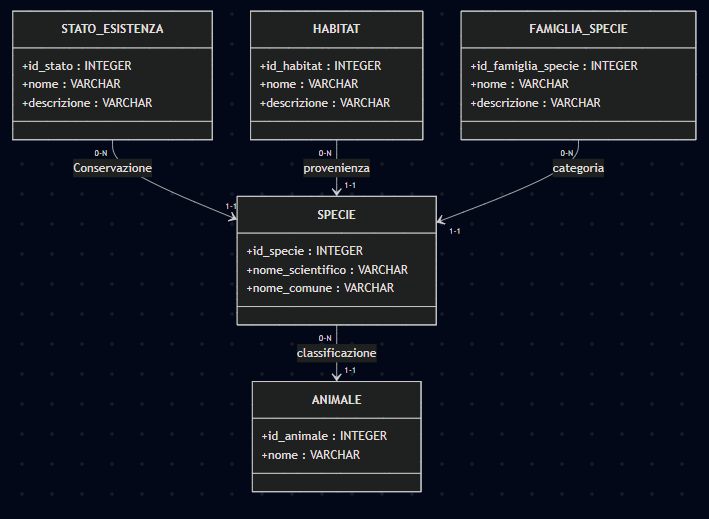
\includegraphics[width=0.6\textwidth]{uml/zoologia.png}
    \caption {schema concettuale}

    \label{fig:zoologia}
\end{figure}

\subsection*{Gestione degli spazi}
\textbf{Area} contiene uno o più \textbf{Recinti}. Ogni recinto appartiene a una sola area e ha una tipologia.
La presenza storica degli animali nei recinti è modellata tramite \textbf{Storico collocazione}.
\href{https://mermaid.ai/live/edit#pako:eNqNkkFvozAQhf8KmusmEQ6kgA-VEEVbpBQqNruHyhJywUmtxXbkGKlNlP--hiYN3bZSOY2f573PHnOAWjUMMNQt3e1uON1oKogkclg7cZnGzoFIx34_eFNRzaiDnSxfpT_T8qRLJZgV_8RlchufRcGMpqbTfXv--y4ts4TI4yW5TBObUozDNau5NOp7-TXdcib3tBI2jYuvMKvsvqg-YRm-Vd8GjvJ-rQqLKKqkWC6LJH7Iijwd5-6M0rz-GNlQQysu-Z73ezfxKh1vrLlkb_KIFufZXbx8B6DSXrZlY8BgGF6KgDvNCTjT6bWt0RTZ-nx57HSPvKb2AJIR-W4u59ZX22vExdaPqlUbTgfM6UR9G_qP9OlssFOrtlU1NYrIC9D9APzCvVZaWC9MYKN5A9jojk1AMKv2SxhGQ8A8McEIYFs2VP8lYMdiPVsqH5QSZ5tW3eYJ8Jq2O7vqtnb47PTPv6mayYbpRHXSAI7CcAgBfIBnwHP3aoYCzw0WaO4uwvBqAi-AEUIzL0Le3A-CwI_cEB0nsB-w7ixEXrDwfS_yFl7kz6PjPzEiCGE}{link mermeid live editor Schema concettuale Gestione degli spazi}

\begin{figure}[H]
    \centering
    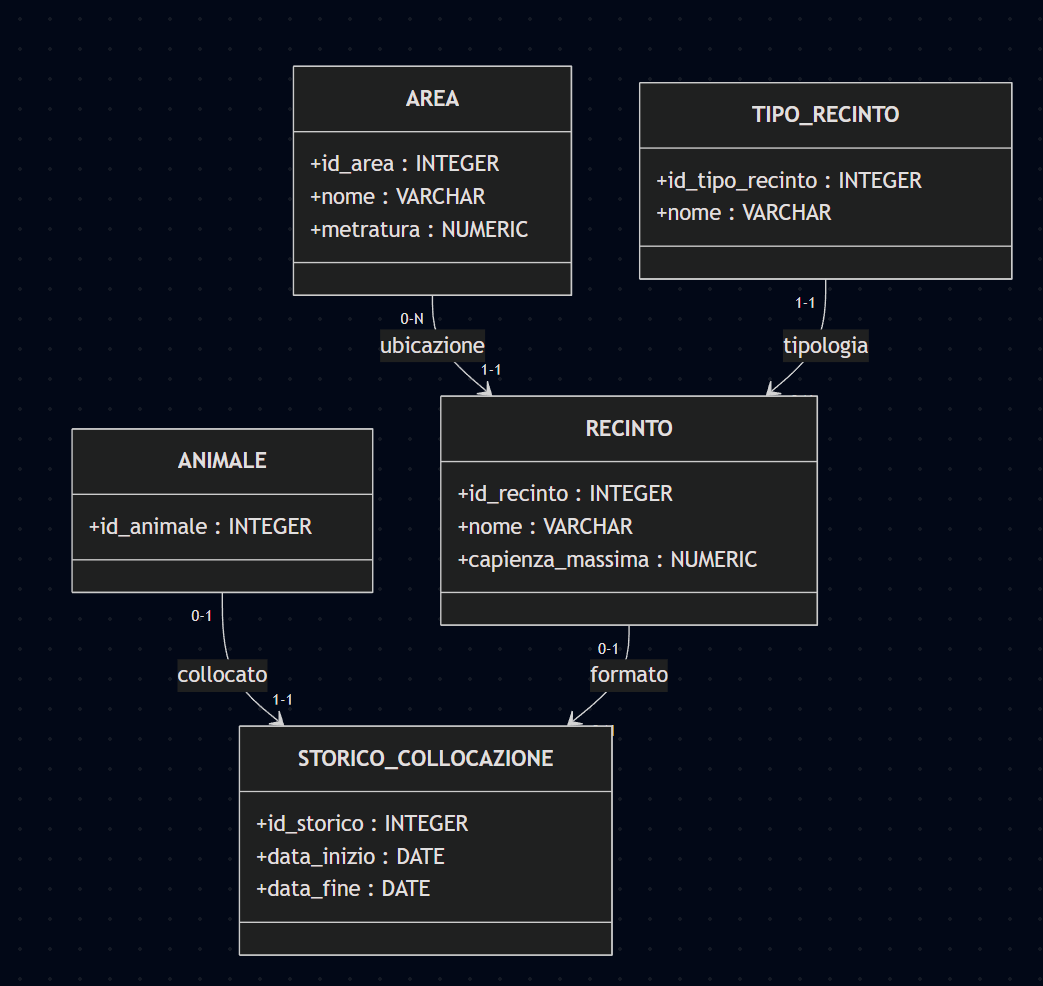
\includegraphics[width=0.6\textwidth]{uml/GestioneSpazi.png}
    \caption {Schema concettuale}

    \label{fig:GestioneSpazi}
\end{figure}



\subsection*{Gestione del personale}
Ogni \textbf{Dipendente} ha una mansione.
I turni vengono registrati tramite \textbf{Turno} e l'andamento degli stipendi è conservato da \textbf{Storico stipendio}.
Un \textbf{Utente} del gestionale è collegato a un dipendente e a un ruolo applicativo.
\href{https://mermaid.ai/live/edit#pako:eNqFU8GOmzAQ_RXka5MIA1mCD5VQgloOIauE7KFCQl7wslbBRgaqlij_XmNI6l22Wk7jeTPvPWbsC8h4TgACWYmbZkdxIXCVsISps7ELH4NoF0RxYFwSZsjvC83TnNaE5YS1xEBGKMFvwXFCGa-G5JN_3H73b8mMF-_z138aez86hYfojUKFWUM5-5xf44nPx-igk7SdYHzGkOMWpwXlI7bz42ACuMApZbSnQz4O98Ep9vePGvhClSEN0tRP8eEYbg_pKVYjC984aVouaDb3UgvS9zyV5EKpRud9IFl0p3dHmlMFTG7GtGbkHL9fV9d-uCpSYVrOdiU6XvL_TNg_Br5OjAXBOq0qva8zAeYySoCxXH6VMVxCGWv3CRlKamjRskPhrWlcKDKaX7wsSMKU_Mg2Mt8KMl4T0eIPqOBdf-yYb0naIK2gz10_3LcZxfwXpvkiA2cZaRoOFqAQNAeoFR1ZgIoIOVd5BGpQCWhfSUUSgGSYY_EzAXJOsqfG7Afn1a1N8K54BegFl408dbVcMZle471keHNiyzvWAgQtx1QkAF3Ab4As82EFXdt019Ay15vNwwL8kVUQrmwP2pbjuq7jmRt4XYBeyZqrDbTdtePYnr22Pcfyrn8Bh8o2gQ}{link mermeid live editor Schema concettuale Gestione del personale}

\begin{figure}[H]
    \centering
    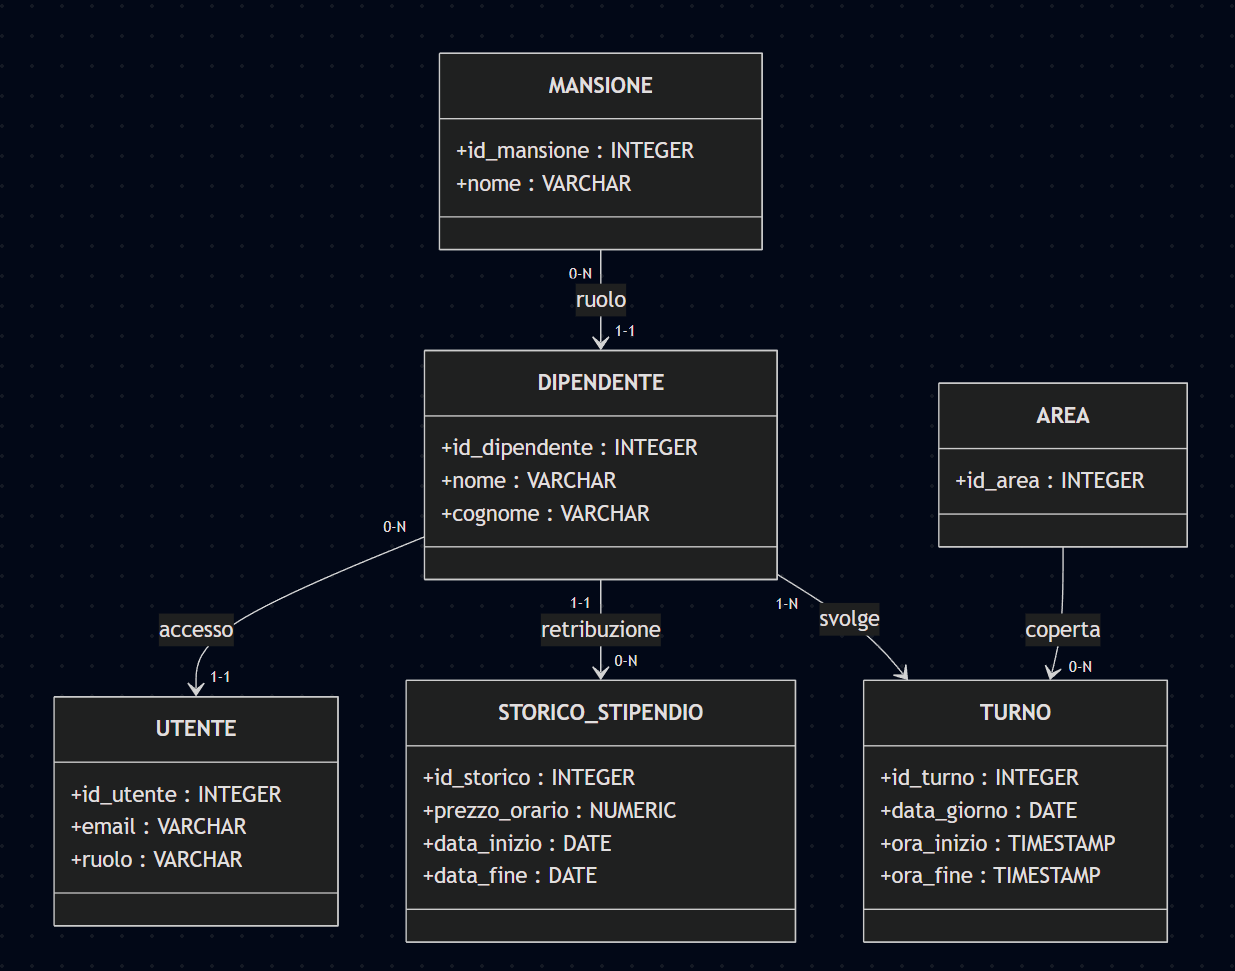
\includegraphics[width=0.6\textwidth]{uml/gestionePersonale.png}
    \caption {Schema concettuale}
    \label{fig:gestionePersonale}
\end{figure}

\subsection*{Sanità veterinaria}
Le \textbf{Visite mediche} collegano animali e veterinari, con data di inizio, eventuale data di fine, diagnosi, peso e note terapeutiche.
\href{https://mermaid.ai/live/edit#pako:eNqNkW9LwzAQxr9Kubeuo2nXP8sLobRBC67InHshgRHWbAbXpKSpqGPf3axurgqCeXX3PPld7i57WKuKA4b1jrVtLthWs5pKKvvcSctilt4RZ0-lY8-VqFZMiprtuIOdolyQGzKn8nAB8uKelDmxzpCpRMNlxaX5C1sWD8UiXc1IXmTpkHwVrTBsSPVOxQy7eHm6IENjIyT_JdvBpGqFVZfpPLtNz4Ua3iorlo8zMi-ykyiV4SujmTGstk2rIdU3fV4LBc8tKTiue21j5CIb_xwFO5pvuDaKysFq_sN9TQcj2GpRATa64yOoua7ZMYV-RxTMM685BWzDiukXCrZDyzRMPilVnzGtuu0z4A3btTbrGrslfvrrb1Uff0hnqpMGMAoSr68CeA9vgP3EG6M48IIkmsQTP_JH8G5voWAcTFEQhyjyk8SP0WEEH_273ngSJSgKYz-ehkE49ePDJwHfuaE}{link mermeid live editor Schema concettuale Sanità veterinaria}

\begin{figure}[H]
    \centering
    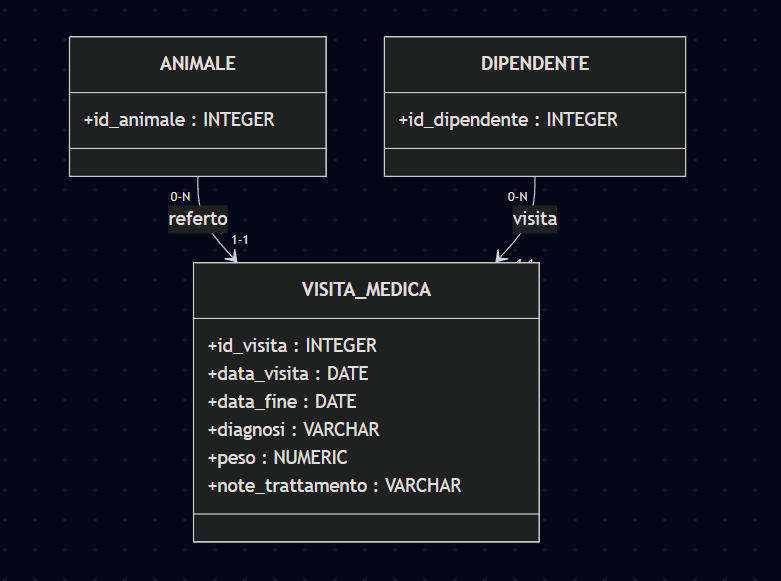
\includegraphics[width=0.6\textwidth]{uml/sanita.png}
    \caption {Schema concettuale}

    \label{fig:sanita}
\end{figure}

\subsection*{Vendita biglietti e contabilità}
La biglietteria è gestita con \textbf{Tipo biglietto}, \textbf{Scontrino}, \textbf{Dettaglio scontrino} e \textbf{Transazione}. Le transazioni sono classificate in entrate o uscite mediante \textbf{Categoria transazione}.
\href{https://mermaid.ai/live/edit#pako:eNqNU99vmzAQ_lfQPW5JFUgawA-TGEEZ0gYVZXuokNANHGot2NQYaUuU_30ObVMSUm08-T5z9_042EMhSgoEii227YphJbHOeMb72kjDuzj_HK6_hkGaxsY-44Z-PrIy_8mqLaNKCYMYYZQG6yB5ueSiphr84SX-F-8VbCTd7Y7vRt-_BUnoZ_zwxnLvx1GahNEZQVsIriTjY4ISFeZYPHWs7elXXhoMuPNKdk0jRhJ4V-cNla3gdDhyoGOlTXraa5xfVVRqu6hdjxU9dcgVUzi6eLadN1ihEmeZXcshTbzo3nsI4ygY8iqJvMUduxDeXyvWOx3YZHUj5DnFKbVTWANSXwPrOAm9_B36AhWthGT4f5s-U9TzvIWZwWwaZWBMp5_02Zya-nwtdGIUQttoWW864xef4WjMh3fnKJRss8F_yxiaJwbjhc5GaOYBfGwzL9qup6cH1E2nnncGE6gkK4Eo2dEJ1FTWeCyhzzgD9UhrmgHRxxLlrwx0bLqnQf4gRP3aJkVXPQLZ4LbVVdfoddKX3_WESspLKn3RcQXEtK1lPwXIHn4DmVvuzWJhWrZtOXPLWdgT-APE1qDjWvbcNpemq_HDBHY97exmuXQdc2bOraXl2O7t7eEvxnZCsw}{link mermeid live editor Schema concettuale Vendita biglietti e contabilità}

\begin{figure}[H]
    \centering
    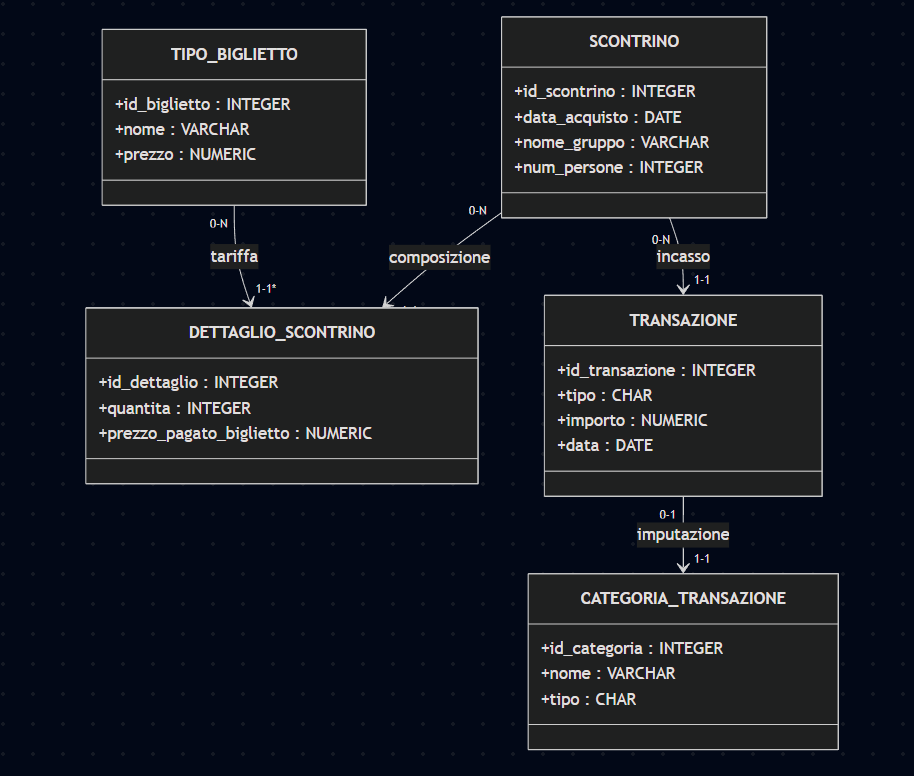
\includegraphics[width=0.6\textwidth]{uml/contabilita.png}
    \caption {Schema concettuale}

    \label{fig:contabilita}
\end{figure}

\subsection*{Approvvigionamenti}
Gli ordini giornalieri di cibo vengono modellati con \textbf{Fornitore}, \textbf{Tipo cibo}, \textbf{Fornitore cibo} e \textbf{Ordine giornaliero}. La relazione tra fornitore e tipo di cibo permette di conoscere i prezzi disponibili.
\href{https://mermaid.ai/live/edit#pako:eNqVU11PgzAU_SvNfXUzK1tg9MEEN1QSBUM2H0yTpUI3G0eLBYyy7L_b4RT3ZWKfeu_JOed-tCtIVMqBQLJkRTEWbKFZRiWVTYyuojgMJlHsoxWVyJwzkc7mSktRKs0RQUE48a_9eAtKlfEZqwWXKTPggxePbjwDrlvFSXAfzb5kp7H3W7YUudpqV5od1f5LcxRcRgdyiXhS_1H66XdXLte8rjdC4fTOj4PRDieKx0Hoz64Dw_VuAz_eKUPpVMjDSaWsZC029ib-FnitmCyFAV8WB37tNij0uiEF1O1e7NdMUDPDIuFUtoP5TThkvJmF8dMOFHAXm_uRTgnSIuFvJ7021PAUNVGmVS4b5713ccy-LY6gIueJYEtR1-a5KcmhAwstUiClrngHMq4ztgmhWQWF8plnnAIx15TpFwpmpIaTM_moVPZN06paPAOZs2Vhoio3W-LbP_GT1ZtZ6ZGqZAkEu5bdqABZwTuQvuWeDwbYchxr2LeGA6cDH0Ackxy6ltN3sI1dk193oG5se-e27Q5xD2PbcnFvYOP1J_vfFGI}{link mermeid live editor Schema concettuale Approvvigionamenti}

\begin{figure}[H]
    \centering
    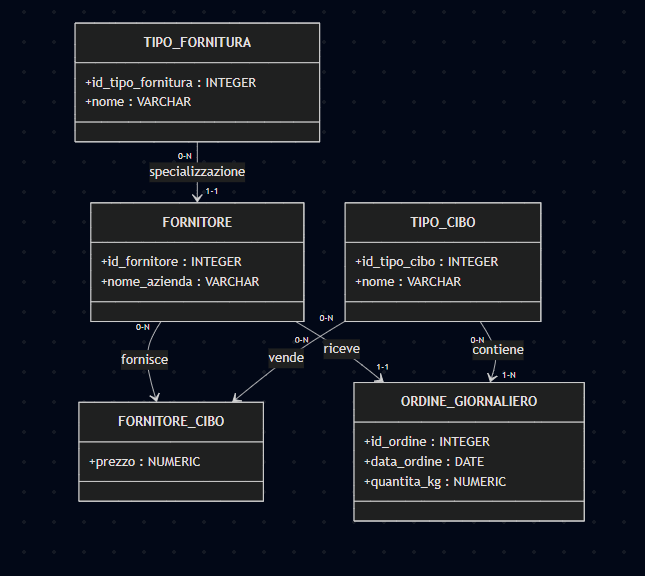
\includegraphics[width=0.6\textwidth]{uml/approvigionamenti.png}
    \caption {Schema concettuale}

    \label{fig:approvigionamenti}
\end{figure}

\section{Schema concettuale finale}

\begin{figure}[H]
    \centering
    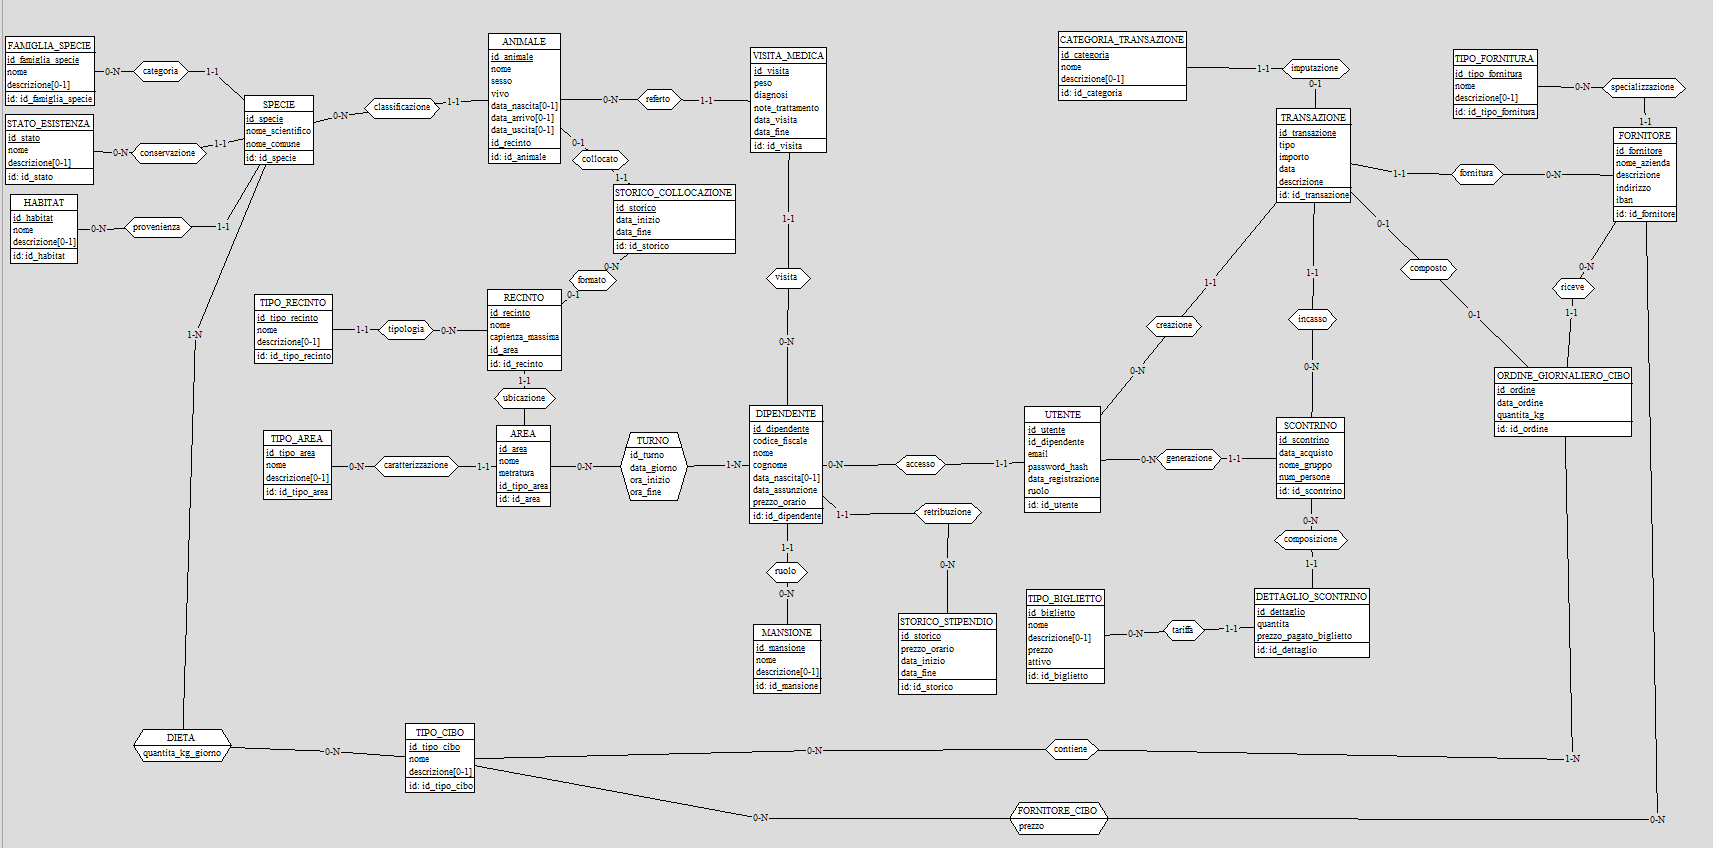
\includegraphics[width=\textwidth]{uml.png}
    \caption{Schema concettuale finale}

    \label{fig:uml}
\end{figure}

\chapter{Progettazione logica}

\section{Stima del volume dei dati}

La tabella seguente riporta una stima ragionata del volume delle istanze per ciascuna
entità/relazione. Le cardinalità sono coerenti con un zoo di dimensione medio-piccola,
con un numero di transazioni e scontrini significativamente maggiore rispetto alle
anagrafiche di base.

\begin{longtable}{L{7cm} C{4cm}}
\toprule
\textbf{Elemento} & \textbf{Volume stimato} \\
\midrule
\endhead
STATO\_ESISTENZA & 6 \\
HABITAT & 7 \\
FAMIGLIA\_SPECIE & 6 \\
TIPO\_AREA & 5 \\
TIPO\_RECINTO & 5 \\
MANSIONE & 6 \\
TIPO\_CIBO & 6 \\
TIPO\_FORNITURA & 5 \\
TIPO\_BIGLIETTO & 6 \\
CATEGORIA\_TRANSAZIONE & 6 \\
SPECIE & 20 \\
DIETA & 40 \\
AREA & 20 \\
RECINTO & 40 \\
ANIMALE & 150 \\
STORICO\_COLLOCAZIONE & 400 \\
DIPENDENTE & 40 \\
STORICO\_STIPENDIO & 80 \\
TURNO & 1500 \\
VISITA\_MEDICA & 500 \\
UTENTE & 40 \\
FORNITORE & 20 \\
FORNITORE\_CIBO & 30 \\
ORDINE\_GIORNALIERO & 8000 \\
SCONTRINO & 120000 \\
DETTAGLIO\_SCONTRINO & 200000 \\
TRANSAZIONE & 150000 \\
\bottomrule
\end{longtable}

\section{Descrizione delle operazioni principali e stima della loro frequenza}

Le operazioni sono state suddivise in operazioni di consultazione e operazioni di
manutenzione. Le prime sono eseguite frequentemente dagli operatori, le seconde
più raramente dall'amministratore.

\begin{longtable}{L{5cm} C{2.5cm} L{5.7cm}}
\toprule
\textbf{Operazione} & \textbf{Frequenza} & \textbf{Tabelle/relazioni principali} \\
\midrule
\endhead
Vendita di un biglietto & 300/giorno & TIPO\_BIGLIETTO, SCONTRINO, DETTAGLIO\_SCONTRINO, TRANSAZIONE \\
Consultazione saldo e ultime transazioni & 50/giorno & TRANSAZIONE, CATEGORIA\_TRANSAZIONE \\
Statistiche biglietteria & 20/giorno & SCONTRINO, DETTAGLIO\_SCONTRINO, TIPO\_BIGLIETTO \\
Consultazione anagrafica animali & 200/giorno & ANIMALE, SPECIE, RECINTO, STORICO\_COLLOCAZIONE \\
Inserimento / modifica animale & 5/settimana & ANIMALE, SPECIE, RECINTO, STORICO\_COLLOCAZIONE \\
Inserimento visita medica & 10/settimana & VISITA\_MEDICA, ANIMALE, DIPENDENTE \\
Gestione turni & 20/settimana & TURNO, DIPENDENTE, AREA \\
Registrazione ordine giornaliero & 5/giorno & FORNITORE, TIPO\_CIBO, FORNITORE\_CIBO, ORDINE\_GIORNALIERO, TRANSAZIONE \\
Aggiornamento classificazioni & 1/mese & STATO\_ESISTENZA, HABITAT, FAMIGLIA\_SPECIE \\
Aggiornamento aree/recinti & 2/mese & AREA, TIPO\_AREA, RECINTO, TIPO\_RECINTO \\
Aggiornamento tipi biglietto & 1/mese & TIPO\_BIGLIETTO \\
\bottomrule
\end{longtable}

\section{Schemi di navigazione e tabelle degli accessi}

\subsection{Schemi di navigazione}

\begin{itemize}[itemsep=2pt]
    \item \textbf{Vendita biglietti}: selezione del tipo di biglietto, creazione dello scontrino, inserimento del dettaglio e della transazione.
    \item \textbf{Saldo amministrativo}: lettura delle transazioni, aggregazione delle entrate e delle uscite, visualizzazione delle ultime movimentazioni.
    \item \textbf{Statistiche biglietteria}: lettura di scontrini e dettagli, raggruppamento per giorno, settimana o mese.
    \item \textbf{Animali}: ricerca per specie e collocazione attuale nel recinto.
    \item \textbf{Visite mediche}: lettura di animali e veterinari, inserimento o aggiornamento delle visite.
    \item \textbf{Ordini giornalieri}: scelta del fornitore, scelta del tipo di cibo disponibile e registrazione dell'ordine.
    \item \textbf{Gestione struttura}: manutenzione di aree, recinti e classificazioni.
\end{itemize}

\subsection{Tabella degli accessi}

\begin{longtable}{L{5cm} C{1.5cm} C{1.8cm} C{3.5cm} C{2.8cm}}
\toprule
\textbf{Operazione} & \textbf{Letture} & \textbf{Scritture} & \textbf{Accessi principali} & \textbf{Osservazioni} \\
\midrule
\endhead
Vendita biglietto & 1 & 3 & TIPO\_BIGLIETTO, SCONTRINO, DETTAGLIO\_SCONTRINO, TRANSAZIONE & Operazione frequente e transazionale \\
Saldo amministrativo & 2 & 0 & TRANSAZIONE, CATEGORIA\_TRANSAZIONE & Richiede scansione e aggregazione \\
Statistiche biglietteria & 3 & 0 & SCONTRINO, DETTAGLIO\_SCONTRINO, TIPO\_BIGLIETTO & Usa raggruppamenti temporali \\
Consultazione animali & 4 & 0 & ANIMALE, SPECIE, RECINTO, STORICO\_COLLOCAZIONE & Accesso prevalentemente in lettura \\
Inserimento animale & 4 & 1 & ANIMALE, RECINTO, SPECIE, STORICO\_COLLOCAZIONE & Eventuale aggiornamento storico \\
Inserimento visita medica & 3 & 1 & VISITA\_MEDICA, ANIMALE, DIPENDENTE & Integrazione con ruolo veterinario \\
Ordine giornaliero & 4 & 2 & FORNITORE, TIPO\_CIBO, FORNITORE\_CIBO, ORDINE\_GIORNALIERO, TRANSAZIONE & Scrittura sia contabile sia logistica \\
Gestione turni & 3 & 1 & TURNO, DIPENDENTE, AREA & Usata dal personale amministrativo \\
\bottomrule
\end{longtable}

\section{Raffinamento dello schema}

Il raffinamento dello schema ha portato alle seguenti scelte:

\begin{itemize}[itemsep=2pt]
    \item tutti gli oggetti principali sono identificati da chiavi surrogate di tipo intero;
    \item le informazioni ripetitive sono normalizzate in tabelle di dominio (tipo area, tipo recinto, categoria transazione, ecc.);
    \item le informazioni storiche sono separate dalle entità correnti;
    \item i legami molti-a-molti sono tradotti tramite tabelle di associazione;
    \item i dati contabili sono separati dai dati operativi.
\end{itemize}

\subsection{Eliminazione di attributi composti e gerarchie}

Nel modello relazionale non sono stati mantenuti attributi composti; gli eventuali
dettagli compositi sono stati scomposti in campi elementari. Inoltre, le gerarchie
concettuali sono state assorbite in tabelle separate di supporto, evitando la
presenza di specializzazioni esplicite nel modello fisico.

\subsection{Scelta delle chiavi}

La scelta delle chiavi è stata guidata da semplicità e stabilità:
\begin{itemize}[itemsep=2pt]
    \item \texttt{id\_animale}, \texttt{id\_specie}, \texttt{id\_recinto}, \texttt{id\_area}, \texttt{id\_dipendente}, \texttt{id\_utente} e le altre chiavi numeriche sono usate come identificatori primari;
    \item per alcune tabelle di dominio è possibile imporre un vincolo di unicità sul nome, quando il dominio lo consente;
    \item le associazioni storiche usano chiavi tecniche che semplificano gli aggiornamenti.
\end{itemize}

\section{Analisi delle ridondanze}

Nel modello logico sono state individuate alcune informazioni che presentano carattere
ridondante o che potrebbero apparire tali a una prima lettura. Per ciascuna si fornisce
una giustificazione progettuale e, dove si tratta di un attributo derivabile, un'analisi
quantitativa degli accessi secondo il metodo delle tabelle degli accessi: ogni scrittura
conta~2, ogni lettura conta~1.

% ===========================================================
\subsection*{Ridondanza 1 -- \texttt{vivo} in ANIMALE}
% ===========================================================

\subsubsection*{Descrizione}

L'attributo \texttt{vivo} (booleano) nella tabella \texttt{ANIMALE} indica se
l'animale è attualmente presente e in vita. Questo valore è \emph{derivabile}
dallo storico delle collocazioni: un animale si considera in vita se esiste almeno
una riga in \texttt{STORICO\_COLLOCAZIONE} con \texttt{data\_fine} \texttt{NULL}.
Tuttavia, navigare lo storico per rispondere a questa domanda introduce un costo
aggiuntivo che si paga su ogni consultazione dell'anagrafica.

Esiste inoltre una seconda informazione apparentemente sovrapposta: \texttt{data\_uscita}
in \texttt{ANIMALE}. Le due informazioni \emph{non sono ridondanti tra loro}: il
flag \texttt{vivo} descrive lo stato corrente (presente/assente dallo zoo),
mentre \texttt{data\_uscita} conserva la data precisa del trasferimento o del
decesso, consentendo di ricostruire la cronologia. Un animale può risultare
\texttt{vivo = false} senza avere una \texttt{data\_uscita} valorizzata (dato mancante)
e viceversa. La coppia è necessaria per distinguere animale presente, animale
trasferito e animale deceduto.

\subsubsection*{Operazioni pertinenti}

\begin{enumerate}[itemsep=2pt]
  \item \textbf{Consultazione anagrafica animali} (200/giorno): recupero dell'elenco
        degli animali con il loro stato corrente.
  \item \textbf{Aggiornamento dello stato di vita} (5/settimana $\approx$ 1/giorno):
        quando un animale muore o viene trasferito, il flag va aggiornato e
        contestualmente va chiusa la riga aperta in \texttt{STORICO\_COLLOCAZIONE}.
\end{enumerate}

\subsubsection*{Dati di volume utili}
\begin{itemize}[itemsep=2pt]
  \item ANIMALE: 150 istanze
  \item STORICO\_COLLOCAZIONE: 400 istanze
  \item Collocazioni medie per animale: $400/150 \approx 2{,}7$
\end{itemize}

\subsubsection*{Tabella degli accessi -- con ridondanza}

\begin{longtable}{L{4.5cm} C{2.5cm} C{2cm} C{2cm}}
\toprule
\textbf{Operazione 1} & \textbf{Costrutto} & \textbf{Accessi} & \textbf{Tipo} \\
\midrule
\endhead
ANIMALE & E & 1 & L \\
\midrule
\multicolumn{2}{l}{\textit{Totale pesato}} & \multicolumn{2}{r}{$1$} \\
\bottomrule
\end{longtable}

\begin{longtable}{L{4.5cm} C{2.5cm} C{2cm} C{2cm}}
\toprule
\textbf{Operazione 2 (aggiornamento)} & \textbf{Costrutto} & \textbf{Accessi} & \textbf{Tipo} \\
\midrule
\endhead
ANIMALE & E & 1 & L \\
ANIMALE & E & 1 & S \\
STORICO\_COLLOCAZIONE & R & 1 & L \\
STORICO\_COLLOCAZIONE & R & 1 & S \\
\midrule
\multicolumn{2}{l}{\textit{Totale pesato}} & \multicolumn{2}{r}{$2\mathrm{L} + 2\mathrm{S} = 6$} \\
\bottomrule
\end{longtable}

\begin{longtable}{C{3cm} C{2.5cm} C{3cm} C{3.5cm}}
\toprule
\textbf{Operazione} & \textbf{Costo/occ.} & \textbf{Freq./giorno} & \textbf{Costo/giorno} \\
\midrule
\endhead
1 & 1 & 200 & 200 \\
2 & 6 & 1   & 6   \\
\midrule
\multicolumn{3}{l}{\textbf{Totale}} & \textbf{206} \\
\bottomrule
\end{longtable}

\subsubsection*{Tabella degli accessi -- senza ridondanza}

Senza il flag, la consultazione deve verificare l'esistenza di una riga aperta in
\texttt{STORICO\_COLLOCAZIONE} per ciascun animale.

\begin{longtable}{L{4.5cm} C{2.5cm} C{2cm} C{2cm}}
\toprule
\textbf{Operazione 1} & \textbf{Costrutto} & \textbf{Accessi} & \textbf{Tipo} \\
\midrule
\endhead
ANIMALE & E & 1 & L \\
STORICO\_COLLOCAZIONE & R & 2{,}7 & L \\
\midrule
\multicolumn{2}{l}{\textit{Totale pesato}} & \multicolumn{2}{r}{$3{,}7$} \\
\bottomrule
\end{longtable}

\begin{longtable}{L{4.5cm} C{2.5cm} C{2cm} C{2cm}}
\toprule
\textbf{Operazione 2 (aggiornamento)} & \textbf{Costrutto} & \textbf{Accessi} & \textbf{Tipo} \\
\midrule
\endhead
STORICO\_COLLOCAZIONE & R & 1 & L \\
STORICO\_COLLOCAZIONE & R & 1 & S \\
\midrule
\multicolumn{2}{l}{\textit{Totale pesato}} & \multicolumn{2}{r}{$3$} \\
\bottomrule
\end{longtable}

\begin{longtable}{C{3cm} C{2.5cm} C{3cm} C{3.5cm}}
\toprule
\textbf{Operazione} & \textbf{Costo/occ.} & \textbf{Freq./giorno} & \textbf{Costo/giorno} \\
\midrule
\endhead
1 & 3{,}7 & 200 & 740 \\
2 & 3   & 1   & 3   \\
\midrule
\multicolumn{3}{l}{\textbf{Totale}} & \textbf{743} \\
\bottomrule
\end{longtable}

\subsubsection*{Decisione}

\begin{center}
\begin{tabular}{lcc}
\toprule
 & \textbf{Con ridondanza} & \textbf{Senza ridondanza} \\
\midrule
Costo/giorno & 206 & 743 \\
\bottomrule
\end{tabular}
\end{center}

Il costo con ridondanza è circa \textbf{3,6 volte inferiore}. La consultazione
anagrafica (200/giorno) è l'operazione dominante e beneficia enormemente del flag
diretto. \textbf{Si mantiene \texttt{vivo} come attributo esplicito.}

% ===========================================================
\subsection*{Ridondanza 2 -- \texttt{prezzo\_pagato\_biglietto} in DETTAGLIO\_SCONTRINO}
% ===========================================================

\subsubsection*{Descrizione}

L'attributo \texttt{prezzo\_pagato\_biglietto} in \texttt{DETTAGLIO\_SCONTRINO}
memorizza il prezzo effettivamente corrisposto al momento dell'acquisto. Tale valore
è \emph{nominalmente derivabile} da \texttt{TIPO\_BIGLIETTO.prezzo}, ma questa
derivazione è valida solo se il prezzo non è mai cambiato. I prezzi dei biglietti
variano nel tempo: senza questa memorizzazione esplicita sarebbe impossibile
ricostruire correttamente i ricavi storici, in quanto il prezzo corrente non
rispecchierebbe quello pagato mesi o anni addietro. La ridondanza ha quindi anche
una funzione di \emph{storicizzazione}, non solo di efficienza.

\subsubsection*{Operazioni pertinenti}

\begin{enumerate}[itemsep=2pt]
  \item \textbf{Vendita di un biglietto} (300/giorno): si legge il prezzo corrente
        da \texttt{TIPO\_BIGLIETTO} e lo si copia nel dettaglio scontrino.
  \item \textbf{Statistiche biglietteria} (20/giorno): calcolo del ricavo per periodo
        tramite \texttt{quantita} $\times$ \texttt{prezzo\_pagato\_biglietto}.
  \item \textbf{Aggiornamento del prezzo del biglietto} (1/mese $\approx$ 0{,}033/giorno):
        modifica di \texttt{TIPO\_BIGLIETTO.prezzo}; con ridondanza non richiede
        aggiornamenti ai dettagli storici.
\end{enumerate}

\subsubsection*{Dati di volume utili}
\begin{itemize}[itemsep=2pt]
  \item TIPO\_BIGLIETTO: 6 istanze
  \item DETTAGLIO\_SCONTRINO: 200\,000 istanze
  \item Media righe dettaglio per scontrino: $200\,000 / 120\,000 \approx 1{,}7$
\end{itemize}

\subsubsection*{Tabella degli accessi -- con ridondanza}

\begin{longtable}{L{5.5cm} C{2.5cm} C{2cm} C{2cm}}
\toprule
\textbf{Operazione 1 (vendita)} & \textbf{Costrutto} & \textbf{Accessi} & \textbf{Tipo} \\
\midrule
\endhead
TIPO\_BIGLIETTO & E & 1 & L \\
SCONTRINO & E & 1 & S \\
DETTAGLIO\_SCONTRINO & E & 1 & S \\
TRANSAZIONE & E & 1 & S \\
\midrule
\multicolumn{2}{l}{\textit{Totale pesato}} & \multicolumn{2}{r}{$1\mathrm{L} + 3\mathrm{S} = 7$} \\
\bottomrule
\end{longtable}

\begin{longtable}{L{5.5cm} C{2.5cm} C{2cm} C{2cm}}
\toprule
\textbf{Operazione 2 (statistiche)} & \textbf{Costrutto} & \textbf{Accessi} & \textbf{Tipo} \\
\midrule
\endhead
SCONTRINO & E & 1 & L \\
DETTAGLIO\_SCONTRINO & R & 1{,}7 & L \\
\midrule
\multicolumn{2}{l}{\textit{Totale pesato}} & \multicolumn{2}{r}{$2{,}7$} \\
\bottomrule
\end{longtable}

\begin{longtable}{L{5.5cm} C{2.5cm} C{2cm} C{2cm}}
\toprule
\textbf{Operazione 3 (aggiornamento prezzo)} & \textbf{Costrutto} & \textbf{Accessi} & \textbf{Tipo} \\
\midrule
\endhead
TIPO\_BIGLIETTO & E & 1 & L \\
TIPO\_BIGLIETTO & E & 1 & S \\
\midrule
\multicolumn{2}{l}{\textit{Totale pesato}} & \multicolumn{2}{r}{$3$} \\
\bottomrule
\end{longtable}

\begin{longtable}{C{3cm} C{2.5cm} C{3cm} C{3.5cm}}
\toprule
\textbf{Operazione} & \textbf{Costo/occ.} & \textbf{Freq./giorno} & \textbf{Costo/giorno} \\
\midrule
\endhead
1 & 7     & 300    & 2\,100 \\
2 & 2{,}7 & 20     & 54     \\
3 & 3     & 0{,}033 & 0{,}1  \\
\midrule
\multicolumn{3}{l}{\textbf{Totale}} & \textbf{2\,154} \\
\bottomrule
\end{longtable}

\subsubsection*{Tabella degli accessi -- senza ridondanza}

Senza l'attributo, le statistiche devono raggiungere \texttt{TIPO\_BIGLIETTO}
per ogni dettaglio, con risultati \emph{potenzialmente incorretti} in caso di
variazione del prezzo.

\begin{longtable}{L{5.5cm} C{2.5cm} C{2cm} C{2cm}}
\toprule
\textbf{Operazione 1 (vendita)} & \textbf{Costrutto} & \textbf{Accessi} & \textbf{Tipo} \\
\midrule
\endhead
TIPO\_BIGLIETTO & E & 1 & L \\
SCONTRINO & E & 1 & S \\
DETTAGLIO\_SCONTRINO & E & 1 & S \\
TRANSAZIONE & E & 1 & S \\
\midrule
\multicolumn{2}{l}{\textit{Totale pesato}} & \multicolumn{2}{r}{$7$} \\
\bottomrule
\end{longtable}

\begin{longtable}{L{5.5cm} C{2.5cm} C{2cm} C{2cm}}
\toprule
\textbf{Operazione 2 (statistiche)} & \textbf{Costrutto} & \textbf{Accessi} & \textbf{Tipo} \\
\midrule
\endhead
SCONTRINO & E & 1 & L \\
DETTAGLIO\_SCONTRINO & R & 1{,}7 & L \\
TIPO\_BIGLIETTO & E & 1{,}7 & L \\
\midrule
\multicolumn{2}{l}{\textit{Totale pesato}} & \multicolumn{2}{r}{$4{,}4$} \\
\bottomrule
\end{longtable}

\begin{longtable}{C{3cm} C{2.5cm} C{3cm} C{3.5cm}}
\toprule
\textbf{Operazione} & \textbf{Costo/occ.} & \textbf{Freq./giorno} & \textbf{Costo/giorno} \\
\midrule
\endhead
1 & 7     & 300    & 2\,100 \\
2 & 4{,}4 & 20     & 88     \\
3 & 3     & 0{,}033 & 0{,}1  \\
\midrule
\multicolumn{3}{l}{\textbf{Totale}} & \textbf{2\,188} \\
\bottomrule
\end{longtable}

\subsubsection*{Decisione}

\begin{center}
\begin{tabular}{lcc}
\toprule
 & \textbf{Con ridondanza} & \textbf{Senza ridondanza} \\
\midrule
Costo/giorno & 2\,154 & 2\,188 \\
\bottomrule
\end{tabular}
\end{center}

La differenza di costo è modesta, ma l'eliminazione dell'attributo renderebbe
\textbf{impossibile ricostruire correttamente i ricavi storici} in presenza di
variazioni di prezzo. \textbf{Si mantiene \texttt{prezzo\_pagato\_biglietto}},
classificandolo come ridondanza necessaria per la correttezza dei dati storici
oltre che per una leggera convenienza di accesso.

% ===========================================================
\subsection*{Ridondanza 3 -- \texttt{num\_persone} in SCONTRINO}
% ===========================================================

\subsubsection*{Descrizione}

L'attributo \texttt{num\_persone} nello \texttt{SCONTRINO} indica quante persone
sono incluse nell'acquisto. Potrebbe sembrare derivabile sommando le
\texttt{quantita} dei dettagli: $\texttt{num\_persone} = \sum \texttt{quantita}$.
Tuttavia questa equivalenza non è sempre valida: nel caso di acquisti di gruppo,
il numero di persone del gruppo può includere accompagnatori o partecipanti
con esenzione non conteggiati come biglietti distinti. Il campo ha quindi un
significato semantico autonomo, utile per le statistiche di affluenza e per
i controlli operativi.

\subsubsection*{Operazioni pertinenti}

\begin{enumerate}[itemsep=2pt]
  \item \textbf{Vendita di un biglietto} (300/giorno): scrittura dello scontrino
        con il numero di persone dichiarato al momento dell'acquisto.
  \item \textbf{Statistiche di affluenza} (20/giorno): aggregazione del numero
        totale di visitatori per periodo.
\end{enumerate}

\subsubsection*{Dati di volume utili}
\begin{itemize}[itemsep=2pt]
  \item SCONTRINO: 120\,000 istanze
  \item DETTAGLIO\_SCONTRINO: 200\,000 istanze
  \item Media righe dettaglio per scontrino: $\approx 1{,}7$
\end{itemize}

\subsubsection*{Tabella degli accessi -- con ridondanza}

\begin{longtable}{L{5cm} C{2.5cm} C{2cm} C{2cm}}
\toprule
\textbf{Operazione 1 (vendita)} & \textbf{Costrutto} & \textbf{Accessi} & \textbf{Tipo} \\
\midrule
\endhead
SCONTRINO & E & 1 & S \\
DETTAGLIO\_SCONTRINO & E & 1 & S \\
\midrule
\multicolumn{2}{l}{\textit{Totale pesato}} & \multicolumn{2}{r}{$2\mathrm{S} = 4$} \\
\bottomrule
\end{longtable}

\begin{longtable}{L{5cm} C{2.5cm} C{2cm} C{2cm}}
\toprule
\textbf{Operazione 2 (statistiche)} & \textbf{Costrutto} & \textbf{Accessi} & \textbf{Tipo} \\
\midrule
\endhead
SCONTRINO & E & 1 & L \\
\midrule
\multicolumn{2}{l}{\textit{Totale pesato}} & \multicolumn{2}{r}{$1$} \\
\bottomrule
\end{longtable}

\begin{longtable}{C{3cm} C{2.5cm} C{3cm} C{3.5cm}}
\toprule
\textbf{Operazione} & \textbf{Costo/occ.} & \textbf{Freq./giorno} & \textbf{Costo/giorno} \\
\midrule
\endhead
1 & 4 & 300 & 1\,200 \\
2 & 1 & 20  & 20     \\
\midrule
\multicolumn{3}{l}{\textbf{Totale}} & \textbf{1\,220} \\
\bottomrule
\end{longtable}

\subsubsection*{Tabella degli accessi -- senza ridondanza}

\begin{longtable}{L{5cm} C{2.5cm} C{2cm} C{2cm}}
\toprule
\textbf{Operazione 1 (vendita)} & \textbf{Costrutto} & \textbf{Accessi} & \textbf{Tipo} \\
\midrule
\endhead
SCONTRINO & E & 1 & S \\
DETTAGLIO\_SCONTRINO & E & 1 & S \\
\midrule
\multicolumn{2}{l}{\textit{Totale pesato}} & \multicolumn{2}{r}{$4$} \\
\bottomrule
\end{longtable}

\begin{longtable}{L{5cm} C{2.5cm} C{2cm} C{2cm}}
\toprule
\textbf{Operazione 2 (statistiche)} & \textbf{Costrutto} & \textbf{Accessi} & \textbf{Tipo} \\
\midrule
\endhead
SCONTRINO & E & 1 & L \\
DETTAGLIO\_SCONTRINO & R & 1{,}7 & L \\
\midrule
\multicolumn{2}{l}{\textit{Totale pesato}} & \multicolumn{2}{r}{$2{,}7$} \\
\bottomrule
\end{longtable}

\begin{longtable}{C{3cm} C{2.5cm} C{3cm} C{3.5cm}}
\toprule
\textbf{Operazione} & \textbf{Costo/occ.} & \textbf{Freq./giorno} & \textbf{Costo/giorno} \\
\midrule
\endhead
1 & 4   & 300 & 1\,200 \\
2 & 2{,}7 & 20 & 54     \\
\midrule
\multicolumn{3}{l}{\textbf{Totale}} & \textbf{1\,254} \\
\bottomrule
\end{longtable}

\subsubsection*{Decisione}

\begin{center}
\begin{tabular}{lcc}
\toprule
 & \textbf{Con ridondanza} & \textbf{Senza ridondanza} \\
\midrule
Costo/giorno & 1\,220 & 1\,254 \\
\bottomrule
\end{tabular}
\end{center}

La differenza numerica è contenuta (34 accessi/giorno), ma il campo ha
un \textbf{significato semantico autonomo} non riducibile alla somma dei dettagli.
\textbf{Si mantiene \texttt{num\_persone} come attributo esplicito.}

% ===========================================================
\subsection*{Considerazioni su STORICO\_COLLOCAZIONE e STORICO\_STIPENDIO}
% ===========================================================

Le entità \texttt{STORICO\_COLLOCAZIONE} e \texttt{STORICO\_STIPENDIO} potrebbero
apparire ridondanti rispetto a una semplice FK diretta sull'animale o sul dipendente.
In realtà non si tratta di ridondanza ma di una precisa \emph{scelta di modellazione
storica}: l'obiettivo non è memorizzare il dato corrente, bensì conservare l'intera
sequenza delle variazioni nel tempo.

\begin{itemize}[itemsep=2pt]
  \item \textbf{STORICO\_COLLOCAZIONE}: memorizza in quale recinto si trovava ciascun
        animale e per quale periodo. Senza questa entità sarebbe impossibile sapere
        dove si trovava un animale in una data passata, quante volte è stato
        spostato o per quanto tempo ha occupato un determinato recinto. Una FK
        diretta da \texttt{ANIMALE} a \texttt{RECINTO} fornirebbe solo la collocazione
        attuale, perdendo tutta la storia degli spostamenti.

  \item \textbf{STORICO\_STIPENDIO}: conserva l'evoluzione della retribuzione oraria
        di ogni dipendente nel tempo. Senza questa entità sarebbe impossibile
        calcolare il costo del lavoro per periodi passati o ricostruire la storia
        contrattuale di un dipendente. Una semplice FK o un campo \texttt{prezzo\_orario}
        direttamente in \texttt{DIPENDENTE} rifletterebbe solo il valore attuale.
\end{itemize}

In entrambi i casi la struttura adottata è quella del \emph{tipo intervallo}:
ogni riga registra un periodo di validità (\texttt{data\_inizio}, \texttt{data\_fine})
e la riga con \texttt{data\_fine} \texttt{NULL} rappresenta la situazione corrente.
Non si tratta quindi di duplicazione, bensì di un \textbf{requisito esplicito di
storicizzazione} emerso dall'intervista con il committente.

% ===========================================================
\subsection*{Considerazioni su \texttt{tipo} e \texttt{id\_categoria} in TRANSAZIONE}
% ===========================================================

In \texttt{TRANSAZIONE} coesistono due informazioni apparentemente simili:
\texttt{tipo} (valori \texttt{ENTRATA}/\texttt{USCITA}) e il riferimento a
\texttt{CATEGORIA\_TRANSAZIONE}. Non si tratta di ridondanza:

\begin{itemize}[itemsep=2pt]
  \item \texttt{tipo} è il \emph{segno contabile} della transazione: determina se
        il movimento incrementa o decrementa il saldo. Viene usato direttamente
        nelle aggregazioni per il calcolo del saldo corrente.

  \item \texttt{id\_categoria} è la \emph{classificazione gestionale}: descrive
        la natura economica della spesa o dell'entrata (es. alimentazione, manutenzione,
        biglietteria, stipendi). Viene usato per le analisi di dettaglio e per
        il budget.
\end{itemize}

Sebbene una categoria possa implicitamente determinare il segno (es. tutte le
vendite biglietti sono entrate), esistono categorie che possono generare movimenti
in entrambe le direzioni (es. rimborsi, rettifiche). Mantenere \texttt{tipo} come
campo autonomo garantisce la correttezza del saldo anche in questi casi limite e
rende le query di aggregazione più semplici ed efficienti, evitando un join aggiuntivo
con \texttt{CATEGORIA\_TRANSAZIONE} per determinare il segno.

% ===========================================================
\subsection*{Riepilogo delle scelte}
% ===========================================================

\begin{longtable}{L{5cm} C{2.2cm} C{2.2cm} C{3.2cm}}
\toprule
\textbf{Elemento} & \textbf{Con rid.} & \textbf{Senza rid.} & \textbf{Decisione} \\
\midrule
\endhead
\texttt{animale.vivo} & 206 & 743 & Mantenuto (efficienza) \\
\texttt{dettaglio\_sco.prezzo\_pagato} & 2\,154 & 2\,188 & Mantenuto (correttezza storica) \\
\texttt{scontrino.num\_persone} & 1\,220 & 1\,254 & Mantenuto (semantica) \\
STORICO\_COLLOCAZIONE & --- & --- & Non è ridondanza (storico) \\
STORICO\_STIPENDIO & --- & --- & Non è ridondanza (storico) \\
\texttt{tipo} in TRANSAZIONE & --- & --- & Non è ridondanza (semantica) \\
\bottomrule
\end{longtable}

\section{Traduzione di entità e associazioni in relazioni}

Lo schema relazionale finale è composto dalle seguenti relazioni.

\begin{longtable}{L{5cm} L{8.5cm}}
\toprule
\textbf{Relazione} & \textbf{Contenuto sintetico} \\
\midrule
\endhead
STATO\_ESISTENZA & dati di classificazione dello stato di conservazione delle specie \\
HABITAT & ambienti naturali di riferimento \\
FAMIGLIA\_SPECIE & famiglie zoologiche \\
TIPO\_AREA & tipologia delle aree dello zoo \\
TIPO\_RECINTO & tipologia dei recinti \\
MANSIONE & ruoli del personale \\
TIPO\_CIBO & categorie di cibo per gli animali \\
TIPO\_FORNITURA & categorie di fornitura \\
TIPO\_BIGLIETTO & tariffe dei biglietti \\
CATEGORIA\_TRANSAZ & classificazione delle transazioni economiche \\
SPECIE & anagrafica delle specie con riferimenti a stato, habitat e famiglia \\
DIETA & fabbisogni alimentari delle specie \\
AREA & aree dello zoo con tipologia associata \\
RECINTO & recinti con area e tipologia \\
ANIMALE & anagrafica degli animali \\
STORICO\_COLLOCAZIO & permanenza degli animali nei recinti nel tempo \\
DIPENDENTE & anagrafica del personale \\
STORICO\_STIPENDIO & variazioni della retribuzione nel tempo \\
TURNO & turni di lavoro del personale \\
VISITA\_MEDICA & visite veterinarie degli animali \\
UTENTE & account del gestionale e ruolo applicativo \\
FORNITORE & anagrafica fornitori \\
FORNITORE\_CIBO & listino cibi per fornitore \\
ORDINE\_GIORNALIERO & ordini di cibo effettuati \\
SCONTRINO & testata di vendita della biglietteria \\
DETTAGLIO\_SCONTRINO & dettaglio dei biglietti venduti \\
TRANSAZIONE & movimenti economici di entrata e uscita \\
\bottomrule
\end{longtable}

\section{Schema relazionale finale}

Il progetto finale, come implementato nel database PostgreSQL, adotta il seguente
insieme di tabelle principali:

\begin{itemize}[itemsep=2pt]
    \item classificazione: \texttt{stato\_esistenza}, \texttt{habitat}, \texttt{famiglia\_specie}, \texttt{specie}, \texttt{dieta};
    \item spazi: \texttt{tipo\_area}, \texttt{tipo\_recinto}, \texttt{area}, \texttt{recinto}, \texttt{storico\_collocazione};
    \item personale: \texttt{mansione}, \texttt{dipendente}, \texttt{storico\_stipendio}, \texttt{turno}, \texttt{utente};
    \item sanità: \texttt{visita\_medica};
    \item contabilità: \texttt{categoria\_transazione}, \texttt{transazione}, \texttt{scontrino}, \texttt{dettaglio\_scontrino}, \texttt{tipo\_biglietto};
    \item approvvigionamenti: \texttt{tipo\_cibo}, \texttt{tipo\_fornitura}, \texttt{fornitore}, \texttt{fornitore\_cibo}, \texttt{ordine\_giornaliero};
    \item altre funzionalità: 
\end{itemize}

\begin{figure}[H]
    \centering
    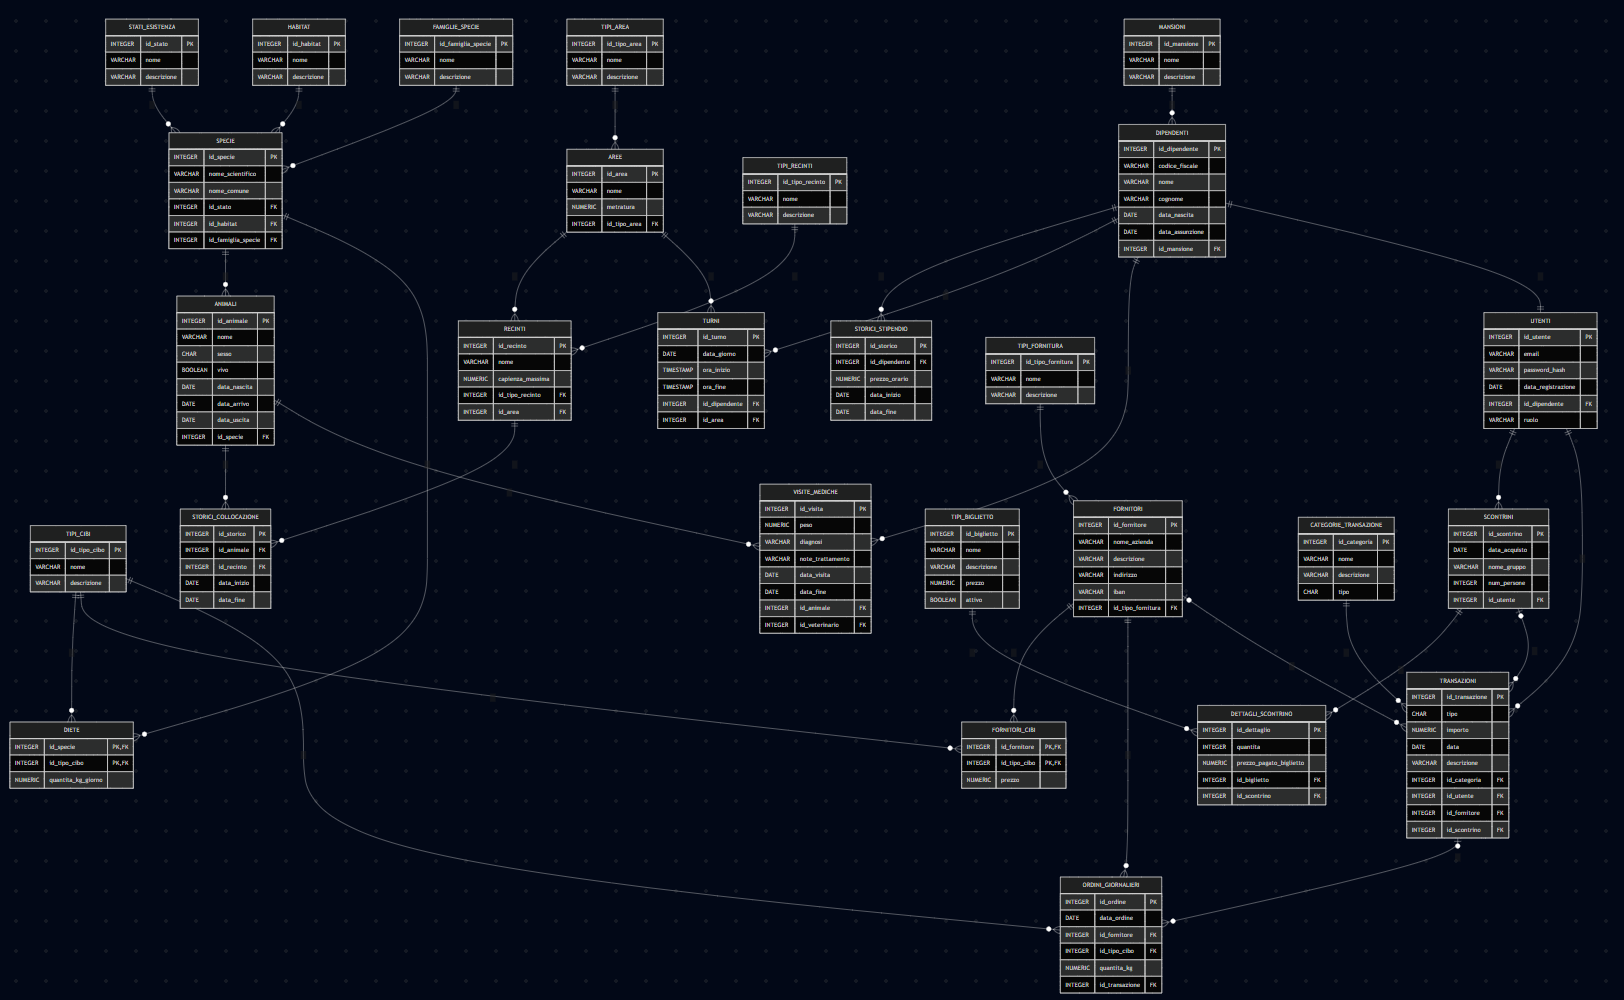
\includegraphics[width=\textwidth]{SchemaRelazionale.png}
    \caption{Schema relazionale finale}

    \label{fig:schema relazionale}
\end{figure}

\centering
Link allo schema relazionale: \href{https://mermaid.ai/live/edit#pako:eNqtWMtS4zgU_ZWU1zRFHjSQnUkMqJo4VGJ6QVHlErZiVI0lt2wzMwGW_SfzZ_Mjc-3E8UuSQ3dYEd3r-zj3Kb0ZHveJMTaImFIcCBw-skfWg7-lYzrItZZo6Vj2g9l72xxnf8h2rGtr0aO-Gyc44b27byXxu7mY3JiLHuMhaZ_6JPYEXVPOtsSPQt-NeYlApULPM36ioOogmq7MGbq-RZa7vLMmyFJoXOGQBi8Uu3FEPEoOotlBd8idoEuk0JnQiLsefToMolr3OrxyY6CyhK6oxxUcHg9TRjRZcfVNG0oFuYl7wbZza4osp9OrI4X0KsI1Hvt-Zi3QpPczxeB2gt0fgRtQLhhvqDdtNDNvVRHEjIb4ZZ9syY9iEscVfC_n81vLtHuv9LVyOjXBXx-DTQxDWBIsI2EhFB-ljW_acLUgzvPUXFimLk-xIPggeQqKVPHcU0cRvJAkAiepwB1Wyx1eQLnYjrY2BeDFDtTw9Or211Q47-EISnaN3RDHMWRhtxeKGpFDtHTmoAXa1_z2dj4xH9DcVlZhwgX0jZrtkhpRqJdZV2YzZRmYMsqKtiCemfYS7FRhHGIWZ4E5SDin6M6yp5Y6oj6NCPOhqcr1wRymHgEvYg_A2dcejwd1wn7NIo5TVnFChYsyCZZO7i2a_14GVKCQ9eBIkPWau1xgIQ_1p5LAuV8oMwB6BatbWYqqdv9Nj5hZsBTN7npgWMuEOrU0Yz_PO6vvO1oix3Jn1hRNblR190pjCHjNnR2kJJbMcR9WPsZjKsu2hLhZM01wCNZKsd6o00fhc6X_ShIiKMvC3obg3tEUV5ooC4uEmL60jyMogr-4yPaR-FnmhCABjQECdZ0oglloECl_4bJBczWHjIS01I7XFWQfzWbZYXbeXCUUr2rbzbVxodkIAQjwFu-htUqkzKdAXEuyjz5hto__rUzYOaPbpase_fY2uOlEDfXzxRTZyL1GYAZsgpYSVMgu2pguZXptiB2md9rdscLKvxbQ3zdprdiELvP7keOo2vtTtqGT5M8WIRXO1UUY-s9uqy2H0GRuOwukbOqxx1kCbUTV2LH3M4XKVt1rApFGEW9LZmnoRkTEqm6wbUHt-woAaQKebmG3ClUfEMUArHxsFlFVjssIB3DrKmPTETlFapXgtRyZAILXUHWW6yxgsdKugB5OSAA7AP7TDMkpWb4383RngnK2V9K8akRDYhVJGkZcSIfdntZKEVAg3ciXz_YATaCaTzfv71--8LfiPWDc--_Xv_U3FyVD86lEylh7bdhyFLdkDcvmHl9RVr6OyDiaN9NCUXZ5rAjJf29pxQ2rqaM4l7PVr_mFx7LbT0VuQ6SOvXE12fm6uz7U-CrnDdnlDl6xo82-WX8VCNWIUscbi6dWlZxXyv3-Xuxz7fCW69FWbrm81JjL4ybfJot0qSVnVciVDHydbDV7bZEtwrmbZvVa2R0XCdIeI00jyrHd-Y2uoxe5UemwFU116yVMTRC5VlzpJ--QWCVwPdLGkREI6hvjRKTkyAiJgDsA_DTySfFoJM8EBpAxhn99LH48Go_sA76JMHvgPCw-EzwNno3xCr_E8CuNYA6Q7SP5jiXb_8WEpywxxoPhKJdhjN-Mv41xf3Dc7w8uTgZn_fP-cHTaB-o_cDwaHl8MT89Ovp6fn5-e9E_OPo6Mda62fzwYDYBvODy56A9GX89HH_8DQ-HeFQ}{link mermeid live editor}



\newpage

\section{Traduzione delle operazioni in query SQL}

% ============================================================
\textbf{SELECT -- Lettura dei dati}
% ============================================================

\subsection{Lettura}
la lettura  di tutti i record (findAll).
Per ogni tabella del sistema è disponibile una query generica di lettura completa, generata dinamicamente dalla classe astratta \texttt{AbstractCrudDao}.
\textbf{la traduzione è quella sotto al codice sql. Non è quella sopra al codice}

\subsubsection*{Animale}
\begin{lstlisting}[style=sqlstyle]
SELECT * FROM animale
\end{lstlisting}
traduzione {Seleziona tutti gli animali presenti nel database.}

\begin{lstlisting}[style=sqlstyle]
SELECT * FROM animale WHERE id_animale = ?
\end{lstlisting}
traduzione {Seleziona un singolo animale identificato dal suo ID.}

\begin{lstlisting}[style=sqlstyle]
SELECT * FROM animale WHERE id_specie = ?
\end{lstlisting}
traduzione {Seleziona tutti gli animali appartenenti a una determinata specie.}

\begin{lstlisting}[style=sqlstyle]
SELECT * FROM animale WHERE vivo = true
\end{lstlisting}
traduzione {Seleziona tutti gli animali attualmente in vita.}

\begin{lstlisting}[style=sqlstyle]
SELECT * FROM animale WHERE vivo = false
\end{lstlisting}
traduzione {Seleziona tutti gli animali deceduti o usciti dallo zoo.}

\subsubsection*{Area}
\begin{lstlisting}[style=sqlstyle]
SELECT * FROM area
\end{lstlisting}
traduzione {Seleziona tutte le aree dello zoo.}

\begin{lstlisting}[style=sqlstyle]
SELECT * FROM area WHERE id_area = ?
\end{lstlisting}
traduzione {Seleziona una singola area identificata dal suo ID.}

\begin{lstlisting}[style=sqlstyle]
SELECT * FROM area WHERE id_tipo_area = ?
\end{lstlisting}
traduzione {Seleziona tutte le aree di un determinato tipo (es. savana, acquatica, ecc.).}

\subsubsection*{Categoria Transazione}
\begin{lstlisting}[style=sqlstyle]
SELECT * FROM categoria_transazione
\end{lstlisting}
traduzione {Seleziona tutte le categorie di transazione disponibili.}

\begin{lstlisting}[style=sqlstyle]
SELECT * FROM categoria_transazione WHERE id_categoria = ?
\end{lstlisting}
traduzione {Seleziona una singola categoria di transazione tramite ID.}

\begin{lstlisting}[style=sqlstyle]
SELECT * FROM categoria_transazione WHERE nome = ?
\end{lstlisting}
traduzione {Seleziona una categoria di transazione cercando per nome.}

\begin{lstlisting}[style=sqlstyle]
SELECT * FROM categoria_transazione WHERE tipo = ?
\end{lstlisting}
traduzione {Seleziona tutte le categorie di transazione di un certo tipo (es. entrata, uscita).}

\subsubsection*{Dettaglio Scontrino}
\begin{lstlisting}[style=sqlstyle]
SELECT * FROM dettaglio_scontrino
\end{lstlisting}
traduzione {Seleziona tutti i dettagli degli scontrini emessi.}

\begin{lstlisting}[style=sqlstyle]
SELECT * FROM dettaglio_scontrino WHERE id_dettaglio = ?
\end{lstlisting}
traduzione {Seleziona un singolo dettaglio di scontrino tramite ID.}

\begin{lstlisting}[style=sqlstyle]
SELECT * FROM dettaglio_scontrino WHERE id_scontrino = ?
\end{lstlisting}
traduzione {Seleziona tutte le righe di dettaglio associate a uno specifico scontrino.}

\begin{lstlisting}[style=sqlstyle]
SELECT * FROM dettaglio_scontrino WHERE id_biglietto = ?
\end{lstlisting}
traduzione {Seleziona tutti i dettagli scontrino che riguardano un determinato tipo di biglietto.}

\subsubsection*{Dieta}
\begin{lstlisting}[style=sqlstyle]
SELECT * FROM dieta
\end{lstlisting}
traduzione {Seleziona tutte le diete definite nel sistema.}

\begin{lstlisting}[style=sqlstyle]
SELECT * FROM dieta WHERE id_specie = ? AND id_tipo_cibo = ?
\end{lstlisting}
traduzione {Seleziona la dieta di una specifica specie per uno specifico tipo di cibo (chiave composta).}

\begin{lstlisting}[style=sqlstyle]
SELECT * FROM dieta WHERE id_specie = ?
\end{lstlisting}
traduzione {Seleziona tutte le voci di dieta associate a una determinata specie animale.}

\begin{lstlisting}[style=sqlstyle]
SELECT * FROM dieta WHERE id_tipo_cibo = ?
\end{lstlisting}
traduzione {Seleziona tutte le diete che prevedono un determinato tipo di cibo.}

\subsubsection*{Dipendente}
\begin{lstlisting}[style=sqlstyle]
SELECT * FROM dipendente
\end{lstlisting}
traduzione {Seleziona tutti i dipendenti dello zoo.}

\begin{lstlisting}[style=sqlstyle]
SELECT * FROM dipendente WHERE id_dipendente = ?
\end{lstlisting}
traduzione {Seleziona un singolo dipendente tramite il suo ID.}

\begin{lstlisting}[style=sqlstyle]
SELECT * FROM dipendente WHERE codice_fiscale = ?
\end{lstlisting}
traduzione {Seleziona un dipendente cercando per codice fiscale.}

\begin{lstlisting}[style=sqlstyle]
SELECT * FROM dipendente WHERE id_mansione = ?
\end{lstlisting}
traduzione {Seleziona tutti i dipendenti che ricoprono una determinata mansione.}

\subsubsection*{Famiglia Specie}
\begin{lstlisting}[style=sqlstyle]
SELECT * FROM famiglia_specie
\end{lstlisting}
traduzione {Seleziona tutte le famiglie tassonomiche presenti nel sistema.}

\begin{lstlisting}[style=sqlstyle]
SELECT * FROM famiglia_specie WHERE id_famiglia_specie = ?
\end{lstlisting}
traduzione {Seleziona una singola famiglia tassonomica tramite ID.}

\begin{lstlisting}[style=sqlstyle]
SELECT * FROM famiglia_specie WHERE nome = ?
\end{lstlisting}
traduzione {Seleziona una famiglia tassonomica cercando per nome.}

\subsubsection*{Fornitore}
\begin{lstlisting}[style=sqlstyle]
SELECT * FROM fornitore
\end{lstlisting}
traduzione {Seleziona tutti i fornitori registrati nel sistema.}

\begin{lstlisting}[style=sqlstyle]
SELECT * FROM fornitore WHERE id_fornitore = ?
\end{lstlisting}
traduzione {Seleziona un singolo fornitore tramite ID.}

\begin{lstlisting}[style=sqlstyle]
SELECT * FROM fornitore WHERE id_tipo_fornitura = ?
\end{lstlisting}
traduzione {Seleziona tutti i fornitori che offrono un determinato tipo di fornitura.}

\subsubsection*{Fornitore Cibo}
\begin{lstlisting}[style=sqlstyle]
SELECT * FROM fornitore_cibo
\end{lstlisting}
traduzione {Seleziona tutte le associazioni tra fornitori e tipi di cibo (con i relativi prezzi).}

\begin{lstlisting}[style=sqlstyle]
SELECT * FROM fornitore_cibo WHERE id_fornitore = ? AND id_tipo_cibo = ?
\end{lstlisting}
traduzione {Seleziona il prezzo di un tipo di cibo specifico offerto da uno specifico fornitore (chiave composta).}

\begin{lstlisting}[style=sqlstyle]
SELECT * FROM fornitore_cibo WHERE id_fornitore = ?
\end{lstlisting}
traduzione {Seleziona tutti i cibi forniti da uno specifico fornitore con i relativi prezzi.}

\begin{lstlisting}[style=sqlstyle]
SELECT * FROM fornitore_cibo WHERE id_tipo_cibo = ?
\end{lstlisting}
traduzione {Seleziona tutti i fornitori che vendono un determinato tipo di cibo.}

\subsubsection*{Habitat}
\begin{lstlisting}[style=sqlstyle]
SELECT * FROM habitat
\end{lstlisting}
traduzione {Seleziona tutti gli habitat definiti nel sistema.}

\begin{lstlisting}[style=sqlstyle]
SELECT * FROM habitat WHERE id_habitat = ?
\end{lstlisting}
traduzione {Seleziona un singolo habitat tramite ID.}

\begin{lstlisting}[style=sqlstyle]
SELECT * FROM habitat WHERE nome = ?
\end{lstlisting}
traduzione {Seleziona un habitat cercando per nome.}

\subsubsection*{Mansione}
\begin{lstlisting}[style=sqlstyle]
SELECT * FROM mansione
\end{lstlisting}
traduzione {Seleziona tutte le mansioni disponibili per i dipendenti.}

\begin{lstlisting}[style=sqlstyle]
SELECT * FROM mansione WHERE id_mansione = ?
\end{lstlisting}
traduzione {Seleziona una singola mansione tramite ID.}

\begin{lstlisting}[style=sqlstyle]
SELECT * FROM mansione WHERE nome = ?
\end{lstlisting}
traduzione {Seleziona una mansione cercando per nome.}

\subsubsection*{Ordine Giornaliero}
\begin{lstlisting}[style=sqlstyle]
SELECT * FROM ordine_giornaliero
\end{lstlisting}
traduzione {Seleziona tutti gli ordini giornalieri di cibo.}

\begin{lstlisting}[style=sqlstyle]
SELECT * FROM ordine_giornaliero WHERE id_ordine = ?
\end{lstlisting}
traduzione {Seleziona un singolo ordine giornaliero tramite ID.}

\begin{lstlisting}[style=sqlstyle]
SELECT * FROM ordine_giornaliero WHERE data_ordine = ? ORDER BY id_ordine DESC
\end{lstlisting}
traduzione {Seleziona tutti gli ordini effettuati in una determinata data, ordinati dal più recente.}

\begin{lstlisting}[style=sqlstyle]
SELECT * FROM ordine_giornaliero WHERE id_fornitore = ? ORDER BY data_ordine DESC
\end{lstlisting}
traduzione {Seleziona tutti gli ordini effettuati a uno specifico fornitore, dal più recente.}

\begin{lstlisting}[style=sqlstyle]
SELECT * FROM ordine_giornaliero WHERE id_tipo_cibo = ? ORDER BY data_ordine DESC
\end{lstlisting}
traduzione {Seleziona tutti gli ordini relativi a uno specifico tipo di cibo, dal più recente.}

\begin{lstlisting}[style=sqlstyle]
SELECT * FROM ordine_giornaliero WHERE id_transazione = ? ORDER BY data_ordine DESC
\end{lstlisting}
traduzione {Seleziona tutti gli ordini associati a una determinata transazione finanziaria, dal più recente.}

\subsubsection*{Recinto}
\begin{lstlisting}[style=sqlstyle]
SELECT * FROM recinto
\end{lstlisting}
traduzione {Seleziona tutti i recinti dello zoo.}

\begin{lstlisting}[style=sqlstyle]
SELECT * FROM recinto WHERE id_recinto = ?
\end{lstlisting}
traduzione {Seleziona un singolo recinto tramite ID.}

\begin{lstlisting}[style=sqlstyle]
SELECT * FROM recinto WHERE id_area = ?
\end{lstlisting}
traduzione {Seleziona tutti i recinti appartenenti a una determinata area.}

\begin{lstlisting}[style=sqlstyle]
SELECT * FROM recinto WHERE id_tipo_recinto = ?
\end{lstlisting}
traduzione {Seleziona tutti i recinti di un determinato tipo.}

\begin{lstlisting}[style=sqlstyle]
SELECT * FROM recinto WHERE capienza_massima >= ?
\end{lstlisting}
traduzione {Seleziona tutti i recinti con una capienza massima pari o superiore al valore indicato.}

\subsubsection*{Scontrino}
\begin{lstlisting}[style=sqlstyle]
SELECT * FROM scontrino
\end{lstlisting}
traduzione {Seleziona tutti gli scontrini emessi.}

\begin{lstlisting}[style=sqlstyle]
SELECT * FROM scontrino WHERE id_scontrino = ?
\end{lstlisting}
traduzione {Seleziona un singolo scontrino tramite ID.}

\begin{lstlisting}[style=sqlstyle]
SELECT * FROM scontrino WHERE data_acquisto = ? ORDER BY id_scontrino DESC
\end{lstlisting}
traduzione {Seleziona tutti gli scontrini emessi in una determinata data, dal più recente.}

\begin{lstlisting}[style=sqlstyle]
SELECT * FROM scontrino WHERE id_utente = ? ORDER BY data_acquisto DESC
\end{lstlisting}
traduzione {Seleziona tutti gli scontrini associati a uno specifico utente, dal più recente per data d'acquisto.}

\subsubsection*{Specie}
\begin{lstlisting}[style=sqlstyle]
SELECT * FROM specie
\end{lstlisting}
traduzione {Seleziona tutte le specie animali registrate.}

\begin{lstlisting}[style=sqlstyle]
SELECT * FROM specie WHERE id_specie = ?
\end{lstlisting}
traduzione {Seleziona una singola specie tramite ID.}

\begin{lstlisting}[style=sqlstyle]
SELECT * FROM specie WHERE id_habitat = ?
\end{lstlisting}
traduzione {Seleziona tutte le specie che vivono in un determinato habitat.}

\begin{lstlisting}[style=sqlstyle]
SELECT * FROM specie WHERE id_stato = ?
\end{lstlisting}
traduzione {Seleziona tutte le specie con un determinato stato di esistenza (es. in via di estinzione).}

\begin{lstlisting}[style=sqlstyle]
SELECT * FROM specie WHERE id_famiglia_specie = ?
\end{lstlisting}
traduzione {Seleziona tutte le specie appartenenti a una determinata famiglia tassonomica.}

\subsubsection*{Stato Esistenza}
\begin{lstlisting}[style=sqlstyle]
SELECT * FROM stato_esistenza
\end{lstlisting}
traduzione {Seleziona tutti gli stati di esistenza (es. vulnerabile, endangered, estinto, ecc.).}

\begin{lstlisting}[style=sqlstyle]
SELECT * FROM stato_esistenza WHERE id_stato = ?
\end{lstlisting}
traduzione {Seleziona un singolo stato di esistenza tramite ID.}

\begin{lstlisting}[style=sqlstyle]
SELECT * FROM stato_esistenza WHERE nome = ?
\end{lstlisting}
traduzione {Seleziona uno stato di esistenza cercando per nome.}

\subsubsection*{Storico Collocazione}
\begin{lstlisting}[style=sqlstyle]
SELECT * FROM storico_collocazione
\end{lstlisting}
traduzione {Seleziona l'intero storico delle collocazioni degli animali nei recinti.}

\begin{lstlisting}[style=sqlstyle]
SELECT * FROM storico_collocazione WHERE id_storico = ?
\end{lstlisting}
traduzione {Seleziona un singolo record dello storico tramite ID.}

\begin{lstlisting}[style=sqlstyle]
SELECT * FROM storico_collocazione WHERE id_animale = ? ORDER BY data_inizio DESC
\end{lstlisting}
traduzione {Seleziona tutto lo storico di collocazione di uno specifico animale, dal più recente.}

\begin{lstlisting}[style=sqlstyle]
SELECT * FROM storico_collocazione WHERE id_recinto = ? ORDER BY data_inizio DESC
\end{lstlisting}
traduzione {Seleziona tutto lo storico di occupazione di uno specifico recinto, dal più recente.}

\subsubsection*{Storico Stipendio}
\begin{lstlisting}[style=sqlstyle]
SELECT * FROM storico_stipendio
\end{lstlisting}
traduzione {Seleziona l'intero storico degli stipendi dei dipendenti.}

\begin{lstlisting}[style=sqlstyle]
SELECT * FROM storico_stipendio WHERE id_storico = ?
\end{lstlisting}
traduzione {Seleziona un singolo record dello storico stipendi tramite ID.}

\begin{lstlisting}[style=sqlstyle]
SELECT * FROM storico_stipendio WHERE id_dipendente = ? ORDER BY data_inizio DESC
\end{lstlisting}
traduzione {Seleziona tutto lo storico stipendi di uno specifico dipendente, dal più recente.}

\subsubsection*{Tipo Area}
\begin{lstlisting}[style=sqlstyle]
SELECT * FROM tipo_area
\end{lstlisting}
traduzione {Seleziona tutti i tipi di area disponibili.}

\begin{lstlisting}[style=sqlstyle]
SELECT * FROM tipo_area WHERE id_tipo_area = ?
\end{lstlisting}
traduzione {Seleziona un singolo tipo di area tramite ID.}

\begin{lstlisting}[style=sqlstyle]
SELECT * FROM tipo_area WHERE nome = ?
\end{lstlisting}
traduzione {Seleziona un tipo di area cercando per nome.}

\subsubsection*{Tipo Biglietto}
\begin{lstlisting}[style=sqlstyle]
SELECT * FROM tipo_biglietto
\end{lstlisting}
traduzione {Seleziona tutti i tipi di biglietto definiti nel sistema.}

\begin{lstlisting}[style=sqlstyle]
SELECT * FROM tipo_biglietto WHERE id_biglietto = ?
\end{lstlisting}
traduzione {Seleziona un singolo tipo di biglietto tramite ID.}

\begin{lstlisting}[style=sqlstyle]
SELECT * FROM tipo_biglietto WHERE nome = ?
\end{lstlisting}
traduzione {Seleziona un tipo di biglietto cercando per nome.}

\begin{lstlisting}[style=sqlstyle]
SELECT * FROM tipo_biglietto WHERE attivo = ?
\end{lstlisting}
traduzione {Seleziona tutti i tipi di biglietto attivi (o non attivi) in base al flag booleano.}

\subsubsection*{Tipo Cibo}
\begin{lstlisting}[style=sqlstyle]
SELECT * FROM tipo_cibo
\end{lstlisting}
traduzione {Seleziona tutti i tipi di cibo registrati.}

\begin{lstlisting}[style=sqlstyle]
SELECT * FROM tipo_cibo WHERE id_tipo_cibo = ?
\end{lstlisting}
traduzione {Seleziona un singolo tipo di cibo tramite ID.}

\begin{lstlisting}[style=sqlstyle]
SELECT * FROM tipo_cibo WHERE nome = ?
\end{lstlisting}
traduzione {Seleziona un tipo di cibo cercando per nome.}

\subsubsection*{Tipo Fornitura}
\begin{lstlisting}[style=sqlstyle]
SELECT * FROM tipo_fornitura
\end{lstlisting}
traduzione {Seleziona tutti i tipi di fornitura disponibili.}

\begin{lstlisting}[style=sqlstyle]
SELECT * FROM tipo_fornitura WHERE id_tipo_fornitura = ?
\end{lstlisting}
traduzione {Seleziona un singolo tipo di fornitura tramite ID.}

\begin{lstlisting}[style=sqlstyle]
SELECT * FROM tipo_fornitura WHERE nome = ?
\end{lstlisting}
traduzione {Seleziona un tipo di fornitura cercando per nome.}

\subsubsection*{Tipo Recinto}
\begin{lstlisting}[style=sqlstyle]
SELECT * FROM tipo_recinto
\end{lstlisting}
traduzione {Seleziona tutti i tipi di recinto presenti.}

\begin{lstlisting}[style=sqlstyle]
SELECT * FROM tipo_recinto WHERE id_tipo_recinto = ?
\end{lstlisting}
traduzione {Seleziona un singolo tipo di recinto tramite ID.}

\begin{lstlisting}[style=sqlstyle]
SELECT * FROM tipo_recinto WHERE nome = ?
\end{lstlisting}
traduzione {Seleziona un tipo di recinto cercando per nome.}

\subsubsection*{Transazione}
\begin{lstlisting}[style=sqlstyle]
SELECT * FROM transazione
\end{lstlisting}
traduzione {Seleziona tutte le transazioni finanziarie registrate.}

\begin{lstlisting}[style=sqlstyle]
SELECT * FROM transazione WHERE id_transazione = ?
\end{lstlisting}
traduzione {Seleziona una singola transazione tramite ID.}

\begin{lstlisting}[style=sqlstyle]
SELECT * FROM transazione WHERE tipo = ? ORDER BY data DESC, id_transazione DESC
\end{lstlisting}
traduzione {Seleziona tutte le transazioni di un certo tipo, ordinate per data decrescente.}

\begin{lstlisting}[style=sqlstyle]
SELECT * FROM transazione WHERE data = ? ORDER BY id_transazione DESC
\end{lstlisting}
traduzione {Seleziona tutte le transazioni effettuate in una determinata data, dalla più recente.}

\begin{lstlisting}[style=sqlstyle]
SELECT * FROM transazione WHERE data >= ? AND data <= ? ORDER BY data DESC, id_transazione DESC
\end{lstlisting}
traduzione {Seleziona tutte le transazioni comprese in un intervallo di date, ordinate per data decrescente.}

\begin{lstlisting}[style=sqlstyle]
SELECT * FROM transazione WHERE id_categoria = ? ORDER BY data DESC, id_transazione DESC
\end{lstlisting}
traduzione {Seleziona tutte le transazioni appartenenti a una determinata categoria, ordinate per data decrescente.}

\begin{lstlisting}[style=sqlstyle]
SELECT * FROM transazione WHERE id_utente = ? ORDER BY data DESC, id_transazione DESC
\end{lstlisting}
traduzione {Seleziona tutte le transazioni associate a uno specifico utente, ordinate per data decrescente.}

\begin{lstlisting}[style=sqlstyle]
SELECT * FROM transazione WHERE id_fornitore = ? ORDER BY data DESC, id_transazione DESC
\end{lstlisting}
traduzione {Seleziona tutte le transazioni relative a uno specifico fornitore, ordinate per data decrescente.}

\begin{lstlisting}[style=sqlstyle]
SELECT * FROM transazione WHERE id_scontrino = ? ORDER BY data DESC, id_transazione DESC
\end{lstlisting}
traduzione {Seleziona tutte le transazioni collegate a uno specifico scontrino, ordinate per data decrescente.}

\subsubsection*{Turno}
\begin{lstlisting}[style=sqlstyle]
SELECT * FROM turno
\end{lstlisting}
traduzione {Seleziona tutti i turni lavorativi registrati.}

\begin{lstlisting}[style=sqlstyle]
SELECT * FROM turno WHERE id_turno = ?
\end{lstlisting}
traduzione {Seleziona un singolo turno tramite ID.}

\begin{lstlisting}[style=sqlstyle]
SELECT * FROM turno WHERE data_giorno = ? ORDER BY ora_inizio
\end{lstlisting}
traduzione {Seleziona tutti i turni di un determinato giorno, ordinati per ora di inizio.}

\begin{lstlisting}[style=sqlstyle]
SELECT * FROM turno WHERE data_giorno >= ? AND data_giorno <= ? ORDER BY data_giorno, ora_inizio
\end{lstlisting}
traduzione {Seleziona tutti i turni compresi in un intervallo di date, ordinati per giorno e ora di inizio.}

\begin{lstlisting}[style=sqlstyle]
SELECT * FROM turno WHERE id_dipendente = ? ORDER BY ora_inizio
\end{lstlisting}
traduzione {Seleziona tutti i turni assegnati a uno specifico dipendente, ordinati per ora di inizio.}

\begin{lstlisting}[style=sqlstyle]
SELECT * FROM turno WHERE id_area = ? ORDER BY ora_inizio
\end{lstlisting}
traduzione {Seleziona tutti i turni relativi a una determinata area, ordinati per ora di inizio.}

\subsubsection*{Utente}
\begin{lstlisting}[style=sqlstyle]
SELECT * FROM utente
\end{lstlisting}
traduzione {Seleziona tutti gli utenti registrati nel sistema.}

\begin{lstlisting}[style=sqlstyle]
SELECT * FROM utente WHERE id_utente = ?
\end{lstlisting}
traduzione {Seleziona un singolo utente tramite ID.}

\begin{lstlisting}[style=sqlstyle]
SELECT * FROM utente WHERE email = ?
\end{lstlisting}
traduzione {Seleziona un utente cercando per indirizzo email (usato tipicamente per il login).}

\begin{lstlisting}[style=sqlstyle]
SELECT * FROM utente WHERE ruolo = ?
\end{lstlisting}
traduzione {Seleziona tutti gli utenti che hanno un determinato ruolo nel sistema.}

\begin{lstlisting}[style=sqlstyle]
SELECT * FROM utente WHERE id_dipendente = ?
\end{lstlisting}
traduzione {Seleziona l'utente associato a uno specifico dipendente.}

\subsubsection*{Visita Medica}
\begin{lstlisting}[style=sqlstyle]
SELECT * FROM visita_medica
\end{lstlisting}
traduzione {Seleziona tutte le visite mediche registrate.}

\begin{lstlisting}[style=sqlstyle]
SELECT * FROM visita_medica WHERE id_visita = ?
\end{lstlisting}
traduzione {Seleziona una singola visita medica tramite ID.}

\begin{lstlisting}[style=sqlstyle]
SELECT * FROM visita_medica WHERE id_animale = ? ORDER BY data_visita DESC
\end{lstlisting}
traduzione {Seleziona tutte le visite mediche di uno specifico animale, dalla più recente.}

\begin{lstlisting}[style=sqlstyle]
SELECT * FROM visita_medica WHERE data_visita = ? ORDER BY id_visita DESC
\end{lstlisting}
traduzione {Seleziona tutte le visite mediche effettuate in una determinata data, dalla più recente.}

\begin{lstlisting}[style=sqlstyle]
SELECT * FROM visita_medica WHERE id_veterinario = ? ORDER BY data_visita DESC
\end{lstlisting}
traduzione {Seleziona tutte le visite mediche eseguite da uno specifico veterinario, dalla più recente.}

\subsection{Inserimento}
% ============================================================
\newpage
\textbf{INSERT -- Inserimento dei dati}
% ============================================================

\begin{lstlisting}[style=sqlstyle]
INSERT INTO animale (nome, sesso, vivo, data_nascita, data_arrivo, data_uscita, id_specie)
VALUES (?, ?, ?, ?, ?, ?, ?)
\end{lstlisting}
traduzione {Inserisce un nuovo animale con nome, sesso, stato in vita, date di nascita, arrivo e uscita, e la specie di appartenenza.}

\begin{lstlisting}[style=sqlstyle]
INSERT INTO area (nome, metratura, id_tipo_area) VALUES (?, ?, ?)
\end{lstlisting}
traduzione {Inserisce una nuova area dello zoo specificando il nome, la superficie in metri quadri e il tipo di area.}

\begin{lstlisting}[style=sqlstyle]
INSERT INTO categoria_transazione (nome, descrizione, tipo) VALUES (?, ?, ?)
\end{lstlisting}
traduzione {Inserisce una nuova categoria di transazione con nome, descrizione e tipo (entrata/uscita).}

\begin{lstlisting}[style=sqlstyle]
INSERT INTO dettaglio_scontrino (id_scontrino, id_biglietto, quantita, prezzo_pagato_biglietto)
VALUES (?, ?, ?, ?)
\end{lstlisting}
traduzione {Inserisce una riga di dettaglio in uno scontrino, specificando il biglietto, la quantità acquistata e il prezzo pagato.}

\begin{lstlisting}[style=sqlstyle]
INSERT INTO dieta (id_specie, id_tipo_cibo, quantita_kg_giorno) VALUES (?, ?, ?)
\end{lstlisting}
traduzione {Inserisce una voce di dieta indicando quanti kg al giorno di un determinato cibo una certa specie deve ricevere.}

\begin{lstlisting}[style=sqlstyle]
INSERT INTO dipendente (codice_fiscale, nome, cognome, data_nascita, data_assunzione, id_mansione)
VALUES (?, ?, ?, ?, ?, ?)
\end{lstlisting}
traduzione {Inserisce un nuovo dipendente con i dati anagrafici, la data di assunzione e la mansione assegnata.}

\begin{lstlisting}[style=sqlstyle]
INSERT INTO famiglia_specie (nome, descrizione) VALUES (?, ?)
\end{lstlisting}
traduzione {Inserisce una nuova famiglia tassonomica con nome e descrizione.}

\begin{lstlisting}[style=sqlstyle]
INSERT INTO fornitore (nome_azienda, descrizione, indirizzo, iban, id_tipo_fornitura)
VALUES (?, ?, ?, ?, ?)
\end{lstlisting}
traduzione {Inserisce un nuovo fornitore con ragione sociale, descrizione, indirizzo, coordinate bancarie e tipo di fornitura offerta.}

\begin{lstlisting}[style=sqlstyle]
INSERT INTO fornitore_cibo (id_fornitore, id_tipo_cibo, prezzo) VALUES (?, ?, ?)
\end{lstlisting}
traduzione {Inserisce una nuova associazione fornitore--cibo, indicando il prezzo al kg praticato da quel fornitore per quel cibo.}

\begin{lstlisting}[style=sqlstyle]
INSERT INTO habitat (nome, descrizione) VALUES (?, ?)
\end{lstlisting}
traduzione {Inserisce un nuovo tipo di habitat con nome e descrizione.}

\begin{lstlisting}[style=sqlstyle]
INSERT INTO mansione (nome, descrizione) VALUES (?, ?)
\end{lstlisting}
traduzione {Inserisce una nuova mansione lavorativa con nome e descrizione.}

\begin{lstlisting}[style=sqlstyle]
INSERT INTO ordine_giornaliero (data_ordine, quantita_kg, id_fornitore, id_tipo_cibo, id_transazione)
VALUES (?, ?, ?, ?, ?)
\end{lstlisting}
traduzione {Inserisce un nuovo ordine giornaliero di cibo specificando la data, la quantità in kg, il fornitore, il tipo di cibo e la transazione associata.}

\begin{lstlisting}[style=sqlstyle]
INSERT INTO recinto (nome, capienza_massima, id_area, id_tipo_recinto) VALUES (?, ?, ?, ?)
\end{lstlisting}
traduzione {Inserisce un nuovo recinto con nome, capienza massima, area di appartenenza e tipo di recinto.}

\begin{lstlisting}[style=sqlstyle]
INSERT INTO scontrino (data_acquisto, nome_gruppo, num_persone, id_utente) VALUES (?, ?, ?, ?)
\end{lstlisting}
traduzione {Inserisce un nuovo scontrino con la data di acquisto, il nome del gruppo, il numero di persone e l'utente che ha effettuato l'acquisto.}

\begin{lstlisting}[style=sqlstyle]
INSERT INTO specie (nome_scientifico, nome_comune, id_habitat, id_stato, id_famiglia_specie)
VALUES (?, ?, ?, ?, ?)
\end{lstlisting}
traduzione {Inserisce una nuova specie animale con nome scientifico, nome comune, habitat, stato di esistenza e famiglia tassonomica.}

\begin{lstlisting}[style=sqlstyle]
INSERT INTO stato_esistenza (nome, descrizione) VALUES (?, ?)
\end{lstlisting}
traduzione {Inserisce un nuovo stato di esistenza (es. LC, VU, EN, CR, EX) con nome e descrizione.}

\begin{lstlisting}[style=sqlstyle]
INSERT INTO storico_collocazione (id_animale, id_recinto, data_inizio, data_fine) VALUES (?, ?, ?, ?)
\end{lstlisting}
traduzione {Inserisce una nuova voce nello storico collocazioni, indicando in quale recinto si trovava un animale e per quale periodo.}

\begin{lstlisting}[style=sqlstyle]
INSERT INTO storico_stipendio (id_dipendente, prezzo_orario, data_inizio, data_fine) VALUES (?, ?, ?, ?)
\end{lstlisting}
traduzione {Inserisce una nuova voce nello storico stipendi di un dipendente con il prezzo orario e il periodo di validità.}

\begin{lstlisting}[style=sqlstyle]
INSERT INTO tipo_area (nome, descrizione) VALUES (?, ?)
\end{lstlisting}
traduzione {Inserisce un nuovo tipo di area con nome e descrizione.}

\begin{lstlisting}[style=sqlstyle]
INSERT INTO tipo_biglietto (nome, descrizione, prezzo, attivo) VALUES (?, ?, ?, ?)
\end{lstlisting}
traduzione {Inserisce un nuovo tipo di biglietto con nome, descrizione, prezzo e flag di attivazione.}

\begin{lstlisting}[style=sqlstyle]
INSERT INTO tipo_cibo (nome, descrizione) VALUES (?, ?)
\end{lstlisting}
traduzione {Inserisce un nuovo tipo di cibo con nome e descrizione.}

\begin{lstlisting}[style=sqlstyle]
INSERT INTO tipo_fornitura (nome, descrizione) VALUES (?, ?)
\end{lstlisting}
traduzione {Inserisce un nuovo tipo di fornitura con nome e descrizione.}

\begin{lstlisting}[style=sqlstyle]
INSERT INTO tipo_recinto (nome, descrizione) VALUES (?, ?)
\end{lstlisting}
traduzione {Inserisce un nuovo tipo di recinto con nome e descrizione.}

\begin{lstlisting}[style=sqlstyle]
INSERT INTO transazione (tipo, importo, data, descrizione, id_categoria, id_utente, id_fornitore, id_scontrino)
VALUES (?, ?, ?, ?, ?, ?, ?, ?)
\end{lstlisting}
traduzione {Inserisce una nuova transazione finanziaria specificando tipo, importo, data, descrizione, categoria, utente, fornitore e scontrino associati.}

\begin{lstlisting}[style=sqlstyle]
INSERT INTO turno (data_giorno, ora_inizio, ora_fine, id_dipendente, id_area)
VALUES (?, ?, ?, ?, ?)
\end{lstlisting}
traduzione {Inserisce un nuovo turno lavorativo con il giorno, l'orario di inizio e fine, il dipendente assegnato e l'area di competenza.}

\begin{lstlisting}[style=sqlstyle]
INSERT INTO utente (email, password_hash, data_registrazione, ruolo, id_dipendente)
VALUES (?, ?, ?, ?, ?)
\end{lstlisting}
traduzione {Inserisce un nuovo utente con email, hash della password, data di registrazione, ruolo e il dipendente associato (se presente).}

\begin{lstlisting}[style=sqlstyle]
INSERT INTO visita_medica (peso, diagnosi, note_trattamento, data_visita, data_fine, id_animale, id_veterinario)
VALUES (?, ?, ?, ?, ?, ?, ?)
\end{lstlisting}
traduzione {Inserisce una nuova visita medica con peso rilevato, diagnosi, note di trattamento, date di inizio e fine, l'animale visitato e il veterinario responsabile.}

\subsection{Update}

% ============================================================
\newpage
\textbf{UPDATE -- Aggiornamento dei dati}
% ============================================================

\begin{lstlisting}[style=sqlstyle]
UPDATE animale
SET nome = ?, sesso = ?, vivo = ?, data_nascita = ?, data_arrivo = ?, data_uscita = ?, id_specie = ?
WHERE id_animale = ?
\end{lstlisting}
traduzione {Aggiorna tutti i dati di un animale esistente identificato dal suo ID.}

\begin{lstlisting}[style=sqlstyle]
UPDATE area SET nome = ?, metratura = ?, id_tipo_area = ? WHERE id_area = ?
\end{lstlisting}
traduzione {Aggiorna nome, metratura e tipo di una area esistente.}

\begin{lstlisting}[style=sqlstyle]
UPDATE categoria_transazione SET nome = ?, descrizione = ?, tipo = ? WHERE id_categoria = ?
\end{lstlisting}
traduzione {Aggiorna nome, descrizione e tipo di una categoria di transazione esistente.}

\begin{lstlisting}[style=sqlstyle]
UPDATE dettaglio_scontrino
SET id_scontrino = ?, id_biglietto = ?, quantita = ?, prezzo_pagato_biglietto = ?
WHERE id_dettaglio = ?
\end{lstlisting}
traduzione {Aggiorna i dati di un dettaglio scontrino esistente.}

\begin{lstlisting}[style=sqlstyle]
UPDATE dieta SET id_specie = ?, id_tipo_cibo = ?, quantita_kg_giorno = ?
WHERE id_specie = ? AND id_tipo_cibo = ?
\end{lstlisting}
traduzione {Aggiorna la quantità giornaliera di un cibo per una determinata specie (chiave composta).}

\begin{lstlisting}[style=sqlstyle]
UPDATE dipendente
SET codice_fiscale = ?, nome = ?, cognome = ?, data_nascita = ?, data_assunzione = ?, id_mansione = ?
WHERE id_dipendente = ?
\end{lstlisting}
traduzione {Aggiorna tutti i dati anagrafici e la mansione di un dipendente.}

\begin{lstlisting}[style=sqlstyle]
UPDATE famiglia_specie SET nome = ?, descrizione = ? WHERE id_famiglia_specie = ?
\end{lstlisting}
traduzione {Aggiorna nome e descrizione di una famiglia tassonomica.}

\begin{lstlisting}[style=sqlstyle]
UPDATE fornitore
SET nome_azienda = ?, descrizione = ?, indirizzo = ?, iban = ?, id_tipo_fornitura = ?
WHERE id_fornitore = ?
\end{lstlisting}
traduzione {Aggiorna tutti i dati di un fornitore esistente.}

\begin{lstlisting}[style=sqlstyle]
UPDATE fornitore_cibo SET prezzo = ? WHERE id_fornitore = ? AND id_tipo_cibo = ?
\end{lstlisting}
traduzione {Aggiorna il prezzo praticato da un fornitore per un determinato tipo di cibo (chiave composta).}

\begin{lstlisting}[style=sqlstyle]
UPDATE habitat SET nome = ?, descrizione = ? WHERE id_habitat = ?
\end{lstlisting}
traduzione {Aggiorna nome e descrizione di un habitat.}

\begin{lstlisting}[style=sqlstyle]
UPDATE mansione SET nome = ?, descrizione = ? WHERE id_mansione = ?
\end{lstlisting}
traduzione {Aggiorna nome e descrizione di una mansione.}

\begin{lstlisting}[style=sqlstyle]
UPDATE ordine_giornaliero
SET data_ordine = ?, quantita_kg = ?, id_fornitore = ?, id_tipo_cibo = ?, id_transazione = ?
WHERE id_ordine = ?
\end{lstlisting}
traduzione {Aggiorna tutti i dati di un ordine giornaliero esistente.}

\begin{lstlisting}[style=sqlstyle]
UPDATE recinto SET nome = ?, capienza_massima = ?, id_area = ?, id_tipo_recinto = ?
WHERE id_recinto = ?
\end{lstlisting}
traduzione {Aggiorna nome, capienza, area e tipo di un recinto.}

\begin{lstlisting}[style=sqlstyle]
UPDATE scontrino SET data_acquisto = ?, nome_gruppo = ?, num_persone = ?, id_utente = ?
WHERE id_scontrino = ?
\end{lstlisting}
traduzione {Aggiorna i dati di uno scontrino esistente.}

\begin{lstlisting}[style=sqlstyle]
UPDATE specie
SET nome_scientifico = ?, nome_comune = ?, id_habitat = ?, id_stato = ?, id_famiglia_specie = ?
WHERE id_specie = ?
\end{lstlisting}
traduzione {Aggiorna tutti i dati di una specie animale.}

\begin{lstlisting}[style=sqlstyle]
UPDATE stato_esistenza SET nome = ?, descrizione = ? WHERE id_stato = ?
\end{lstlisting}
traduzione {Aggiorna nome e descrizione di uno stato di esistenza.}

\begin{lstlisting}[style=sqlstyle]
UPDATE storico_collocazione
SET id_animale = ?, id_recinto = ?, data_inizio = ?, data_fine = ?
WHERE id_storico = ?
\end{lstlisting}
traduzione {Aggiorna i dati di una voce dello storico collocazioni (es. per impostare la data di fine).}

\begin{lstlisting}[style=sqlstyle]
UPDATE storico_stipendio
SET id_dipendente = ?, prezzo_orario = ?, data_inizio = ?, data_fine = ?
WHERE id_storico = ?
\end{lstlisting}
traduzione {Aggiorna i dati di una voce dello storico stipendi (es. per chiudere un periodo).}

\begin{lstlisting}[style=sqlstyle]
UPDATE tipo_area SET nome = ?, descrizione = ? WHERE id_tipo_area = ?
\end{lstlisting}
traduzione {Aggiorna nome e descrizione di un tipo di area.}

\begin{lstlisting}[style=sqlstyle]
UPDATE tipo_biglietto SET nome = ?, descrizione = ?, prezzo = ?, attivo = ? WHERE id_biglietto = ?
\end{lstlisting}
traduzione {Aggiorna tutti i dati di un tipo di biglietto, incluso il prezzo e il flag di attivazione.}

\begin{lstlisting}[style=sqlstyle]
UPDATE tipo_cibo SET nome = ?, descrizione = ? WHERE id_tipo_cibo = ?
\end{lstlisting}
traduzione {Aggiorna nome e descrizione di un tipo di cibo.}

\begin{lstlisting}[style=sqlstyle]
UPDATE tipo_fornitura SET nome = ?, descrizione = ? WHERE id_tipo_fornitura = ?
\end{lstlisting}
traduzione {Aggiorna nome e descrizione di un tipo di fornitura.}

\begin{lstlisting}[style=sqlstyle]
UPDATE tipo_recinto SET nome = ?, descrizione = ? WHERE id_tipo_recinto = ?
\end{lstlisting}
traduzione {Aggiorna nome e descrizione di un tipo di recinto.}

\begin{lstlisting}[style=sqlstyle]
UPDATE transazione
SET tipo = ?, importo = ?, data = ?, descrizione = ?, id_categoria = ?, id_utente = ?, id_fornitore = ?, id_scontrino = ?
WHERE id_transazione = ?
\end{lstlisting}
traduzione {Aggiorna tutti i dati di una transazione finanziaria esistente.}

\begin{lstlisting}[style=sqlstyle]
UPDATE turno SET data_giorno = ?, ora_inizio = ?, ora_fine = ?, id_dipendente = ?, id_area = ?
WHERE id_turno = ?
\end{lstlisting}
traduzione {Aggiorna i dati di un turno lavorativo esistente.}

\begin{lstlisting}[style=sqlstyle]
UPDATE utente SET email = ?, password_hash = ?, data_registrazione = ?, ruolo = ?, id_dipendente = ?
WHERE id_utente = ?
\end{lstlisting}
traduzione {Aggiorna tutti i dati di un utente, incluse email, password e ruolo.}

\begin{lstlisting}[style=sqlstyle]
UPDATE visita_medica
SET peso = ?, diagnosi = ?, note_trattamento = ?, data_visita = ?, data_fine = ?, id_animale = ?, id_veterinario = ?
WHERE id_visita = ?
\end{lstlisting}
traduzione {Aggiorna tutti i dati di una visita medica esistente.}

\subsection{Cancellazione}

% ============================================================
\newpage
\textbf{DELETE -- Cancellazione dei dati}
% ============================================================

Le query di cancellazione sono generate dinamicamente dalla classe astratta \texttt{AbstractCrudDao} e \texttt{AbstractCompositeCrudDao}. Di seguito le forme concrete per ogni tabella.

\begin{lstlisting}[style=sqlstyle]
DELETE FROM animale WHERE id_animale = ?
\end{lstlisting}
traduzione {Elimina un animale dal database tramite il suo ID.}

\begin{lstlisting}[style=sqlstyle]
DELETE FROM area WHERE id_area = ?
\end{lstlisting}
traduzione {Elimina un'area tramite il suo ID.}

\begin{lstlisting}[style=sqlstyle]
DELETE FROM categoria_transazione WHERE id_categoria = ?
\end{lstlisting}
traduzione {Elimina una categoria di transazione tramite il suo ID.}

\begin{lstlisting}[style=sqlstyle]
DELETE FROM dettaglio_scontrino WHERE id_dettaglio = ?
\end{lstlisting}
traduzione {Elimina un dettaglio scontrino tramite il suo ID.}

\begin{lstlisting}[style=sqlstyle]
DELETE FROM dieta WHERE id_specie = ? AND id_tipo_cibo = ?
\end{lstlisting}
traduzione {Elimina la voce di dieta di una specie per un determinato tipo di cibo (chiave composta).}

\begin{lstlisting}[style=sqlstyle]
DELETE FROM dipendente WHERE id_dipendente = ?
\end{lstlisting}
traduzione {Elimina un dipendente tramite il suo ID.}

\begin{lstlisting}[style=sqlstyle]
DELETE FROM famiglia_specie WHERE id_famiglia_specie = ?
\end{lstlisting}
traduzione {Elimina una famiglia tassonomica tramite il suo ID.}

\begin{lstlisting}[style=sqlstyle]
DELETE FROM fornitore WHERE id_fornitore = ?
\end{lstlisting}
traduzione {Elimina un fornitore tramite il suo ID.}

\begin{lstlisting}[style=sqlstyle]
DELETE FROM fornitore_cibo WHERE id_fornitore = ? AND id_tipo_cibo = ?
\end{lstlisting}
traduzione {Elimina l'associazione tra un fornitore e un tipo di cibo (chiave composta).}

\begin{lstlisting}[style=sqlstyle]
DELETE FROM habitat WHERE id_habitat = ?
\end{lstlisting}
traduzione {Elimina un habitat tramite il suo ID.}

\begin{lstlisting}[style=sqlstyle]
DELETE FROM mansione WHERE id_mansione = ?
\end{lstlisting}
traduzione {Elimina una mansione tramite il suo ID.}

\begin{lstlisting}[style=sqlstyle]
DELETE FROM ordine_giornaliero WHERE id_ordine = ?
\end{lstlisting}
traduzione {Elimina un ordine giornaliero tramite il suo ID.}

\begin{lstlisting}[style=sqlstyle]
DELETE FROM recinto WHERE id_recinto = ?
\end{lstlisting}
traduzione {Elimina un recinto tramite il suo ID.}

\begin{lstlisting}[style=sqlstyle]
DELETE FROM scontrino WHERE id_scontrino = ?
\end{lstlisting}
traduzione {Elimina uno scontrino tramite il suo ID.}

\begin{lstlisting}[style=sqlstyle]
DELETE FROM specie WHERE id_specie = ?
\end{lstlisting}
traduzione {Elimina una specie animale tramite il suo ID.}

\begin{lstlisting}[style=sqlstyle]
DELETE FROM stato_esistenza WHERE id_stato = ?
\end{lstlisting}
traduzione {Elimina uno stato di esistenza tramite il suo ID.}

\begin{lstlisting}[style=sqlstyle]
DELETE FROM storico_collocazione WHERE id_storico = ?
\end{lstlisting}
traduzione {Elimina una voce dello storico collocazioni tramite il suo ID.}

\begin{lstlisting}[style=sqlstyle]
DELETE FROM storico_stipendio WHERE id_storico = ?
\end{lstlisting}
traduzione {Elimina una voce dello storico stipendi tramite il suo ID.}

\begin{lstlisting}[style=sqlstyle]
DELETE FROM tipo_area WHERE id_tipo_area = ?
\end{lstlisting}
traduzione {Elimina un tipo di area tramite il suo ID.}

\begin{lstlisting}[style=sqlstyle]
DELETE FROM tipo_biglietto WHERE id_biglietto = ?
\end{lstlisting}
traduzione {Elimina un tipo di biglietto tramite il suo ID.}

\begin{lstlisting}[style=sqlstyle]
DELETE FROM tipo_cibo WHERE id_tipo_cibo = ?
\end{lstlisting}
traduzione {Elimina un tipo di cibo tramite il suo ID.}

\begin{lstlisting}[style=sqlstyle]
DELETE FROM tipo_fornitura WHERE id_tipo_fornitura = ?
\end{lstlisting}
traduzione {Elimina un tipo di fornitura tramite il suo ID.}

\begin{lstlisting}[style=sqlstyle]
DELETE FROM tipo_recinto WHERE id_tipo_recinto = ?
\end{lstlisting}
traduzione {Elimina un tipo di recinto tramite il suo ID.}

\begin{lstlisting}[style=sqlstyle]
DELETE FROM transazione WHERE id_transazione = ?
\end{lstlisting}
traduzione {Elimina una transazione finanziaria tramite il suo ID.}

\begin{lstlisting}[style=sqlstyle]
DELETE FROM turno WHERE id_turno = ?
\end{lstlisting}
traduzione {Elimina un turno lavorativo tramite il suo ID.}

\begin{lstlisting}[style=sqlstyle]
DELETE FROM utente WHERE id_utente = ?
\end{lstlisting}
traduzione {Elimina un utente tramite il suo ID.}

\begin{lstlisting}[style=sqlstyle]
DELETE FROM visita_medica WHERE id_visita = ?
\end{lstlisting}
traduzione {Elimina una visita medica tramite il suo ID.}


\chapter{Progettazione dell'applicazione}

\section{Architettura dell'applicazione realizzata}

L'applicazione è stata sviluppata in Java con JavaFX e segue una struttura MVC
piuttosto netta:

\begin{itemize}[itemsep=2pt]
    \item \textbf{View}: definiscono la GUI, le tabelle e i moduli di inserimento;
    \item \textbf{Controller}: collegano gli eventi dell'interfaccia alle operazioni di dominio;
    \item \textbf{Model}: contiene le classi entità e i DAO per l'accesso ai dati;
    \item \textbf{Database}: PostgreSQL eseguito tramite Docker.
\end{itemize}

Le principali scelte architetturali sono:
\begin{itemize}[itemsep=2pt]
    \item \textbf{DAO JDBC}: ogni tabella principale ha il proprio DAO, con metodi per CRUD e ricerche mirate;
    \item \textbf{Password hashing}: le password sono memorizzate come hash bcrypt;
    \item \textbf{Configurazione esterna}: i parametri del DB sono letti da variabili d'ambiente;
    \item \textbf{Navgazione centralizzata}: una finestra principale ospita pannelli diversi in base alla sezione selezionata;
    \item \textbf{Controllo dei ruoli}: il pannello di gestione filtra i tab in base al ruolo dell'utente autenticato.
\end{itemize}

\subsection*{Struttura funzionale dell'interfaccia}

L'interfaccia pubblica comprende:
\begin{itemize}[itemsep=2pt]
    \item Home;
    \item Animali;
    \item Biglietti;
    \item Donazioni;
    \item Login.
\end{itemize}

L’area riservata include i moduli di amministrazione del sistema. La visibilità delle schermate e delle funzionalità disponibili varia in base al ruolo svolto dall’utente all’interno del parco: non tutti gli utenti hanno accesso a tutti i moduli, ma soltanto a quelli pertinenti alle proprie mansioni. Sono previsti quattro profili utente con differenti permessi e livelli di accesso: 
\begin{itemize}
    \renewcommand{\labelitemi}{-}
    \item Amministratore (admin@zoopark.it), password: password123
    \item Operatore di biglietteria (biglietteria@zoopark.it), password: password123
    \item Veterinario (vet.rossi@zoopark.it), password: password123
    \item Guardiano (guardiano@zoopark.it), password: password123
\end{itemize}
L’utente amministratore dispone di accesso completo a tutte le schermate e a tutte le funzionalità del sistema, mentre gli altri utenti visualizzano esclusivamente le sezioni necessarie allo svolgimento delle proprie attività. Per semplicita e scopi didattici è stata assegnata la stessa password a tutti gli utenti e nel database viene salvata l'hash della password.
\newline
Questo è l'elenco di tutte le schermate esistenti:
\begin{itemize}[itemsep=2pt]
    \item saldo e statistiche;
    \item tipi biglietto;
    \item ordini giornalieri;
    \item visite mediche;
    \item turni;
    \item personale;
    \item spese;
    \item animali;
    \item classificazione;
    \item aree;
    \item recinti.
\end{itemize}

\section{Screenshot dell'interfaccia utente}

Le figure seguenti sono predisposte per accogliere alcuni screenshot dell'applicazione
realizzata per aiutare l'utente all'uso dell'applicativo. 

\subsection{Schermata principale}

La schermata principale rappresenta la homepage pubblica del sistema ZooPark. Da questa pagina l'utente può accedere alle informazioni generali del parco, consultare i servizi disponibili e raggiungere l'area riservata tramite l'apposita funzione di login.
\begin{figure}[H]
    \centering
    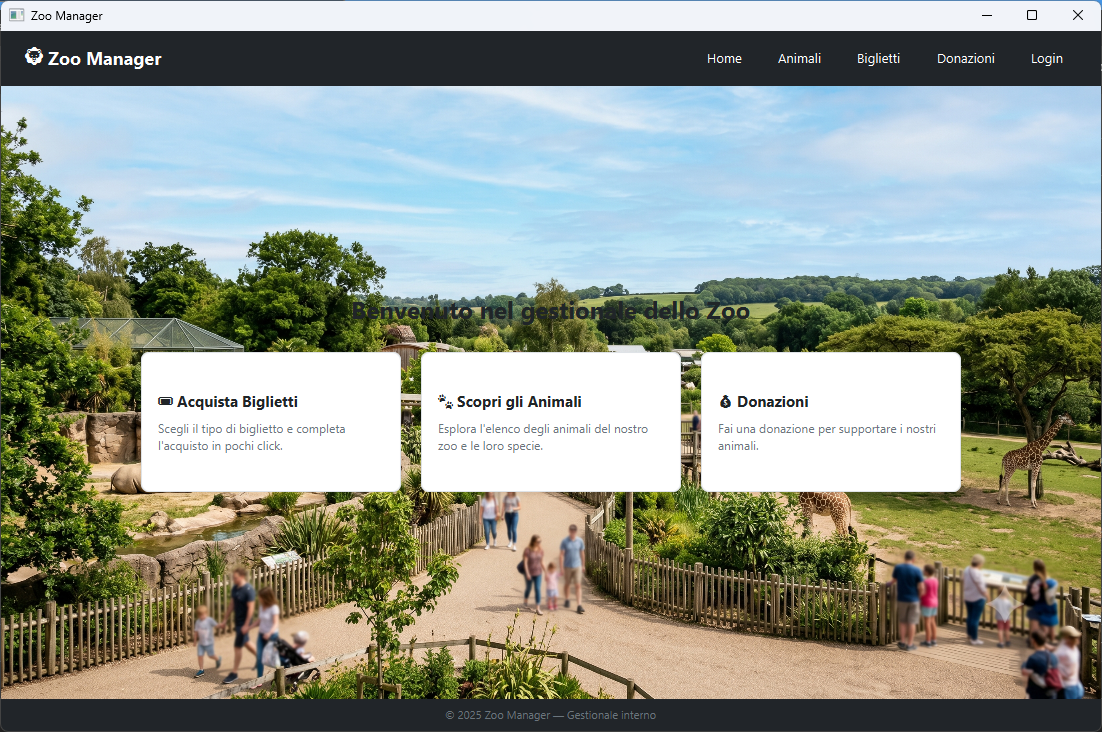
\includegraphics[width=\textwidth]{schermate/principale.png}
    \caption {Immagine della schermata principale}

    \label{fig:schermataPrincipale}
\end{figure}

\subsection{Schermata di login}

La schermata di login consente agli utenti autorizzati di autenticarsi inserendo le proprie credenziali. In base al ruolo associato all'account, il sistema mostrerà funzionalità e sezioni differenti dell'area riservata.

\begin{figure}[H]
    \centering
    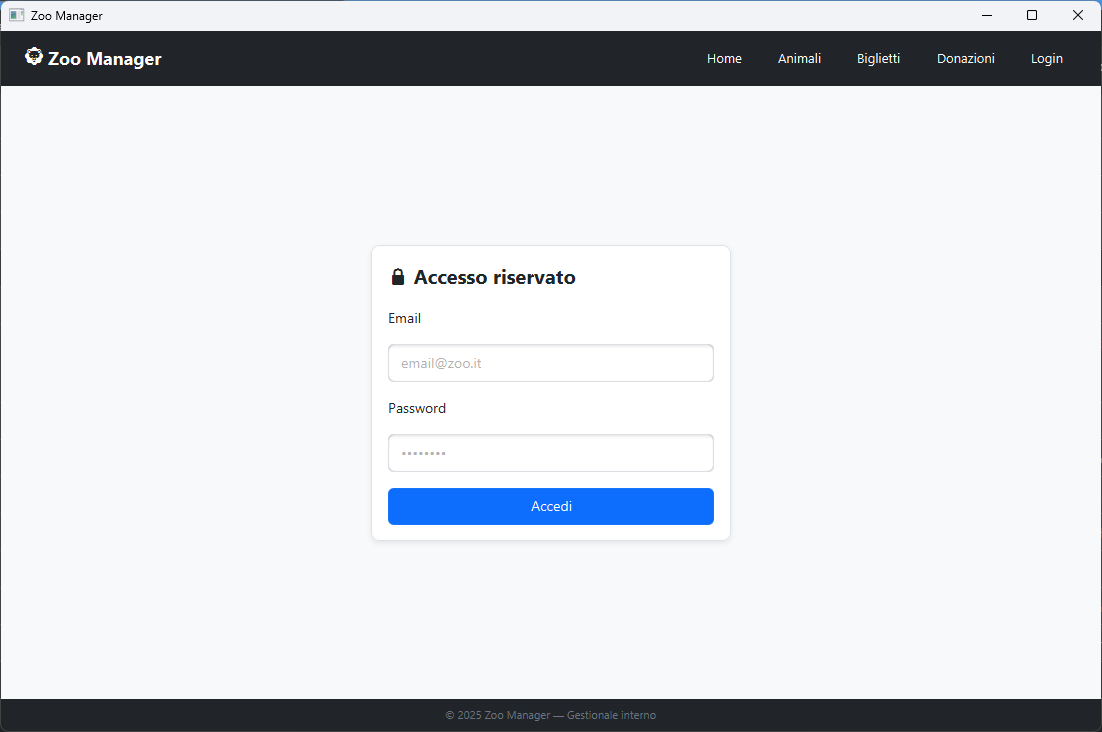
\includegraphics[width=\textwidth]{schermate/login.png}
    \caption {Immagine della schermata di login}

    \label{fig:schermataLogin}
\end{figure}

\subsection{Schermata dal punto di vista di admin}

Una volta effettuato l'accesso come amministratore, vengono rese disponibili tutte le funzionalità del sistema. Questo ruolo dispone di accesso completo ai moduli di gestione degli animali, del personale, delle strutture e delle attività amministrative del parco.

\begin{figure}[H]
    \centering
    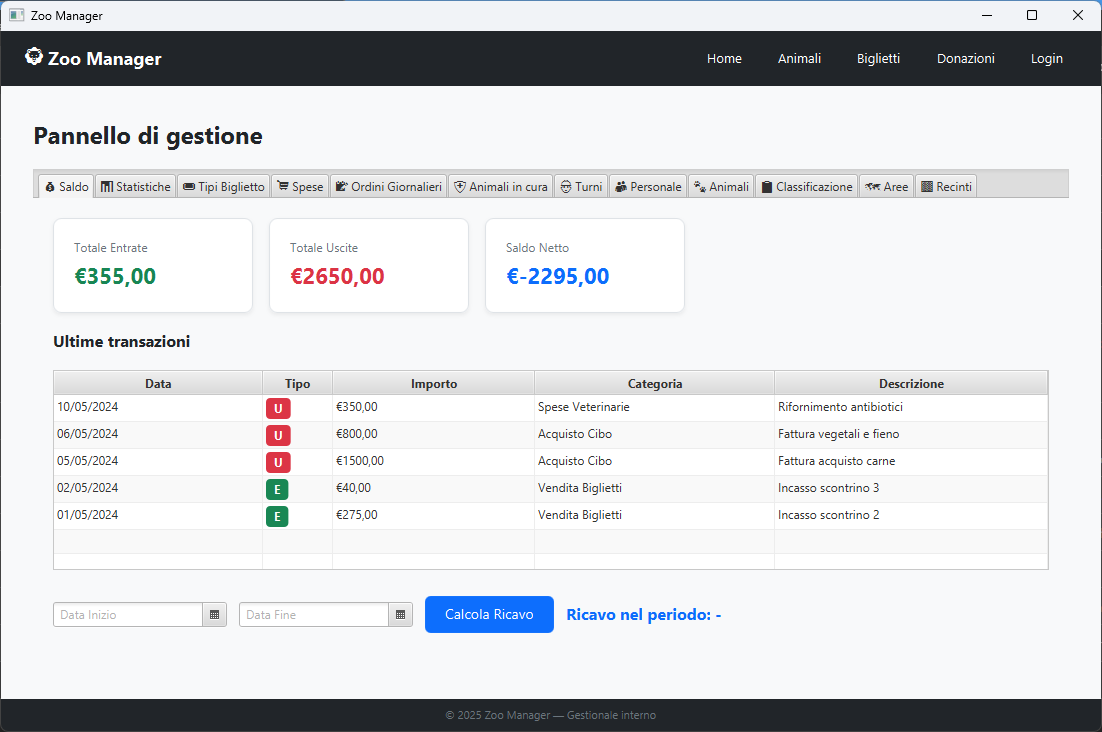
\includegraphics[width=\textwidth]{schermate/loginADMIN.png}
    \caption {Immagine della schermata di loged come admin}

    \label{fig:schermataLogedAdmin}
\end{figure}

\subsection{Schermata dal punto di vista del veterinario}

La schermata visualizzata dal veterinario mostra esclusivamente le funzionalità pertinenti alle sue mansioni. In particolare, il veterinario può consultare e aggiornare le informazioni sanitarie degli animali, senza accedere ai moduli amministrativi riservati ad altri ruoli.

\begin{figure}[H]
    \centering
    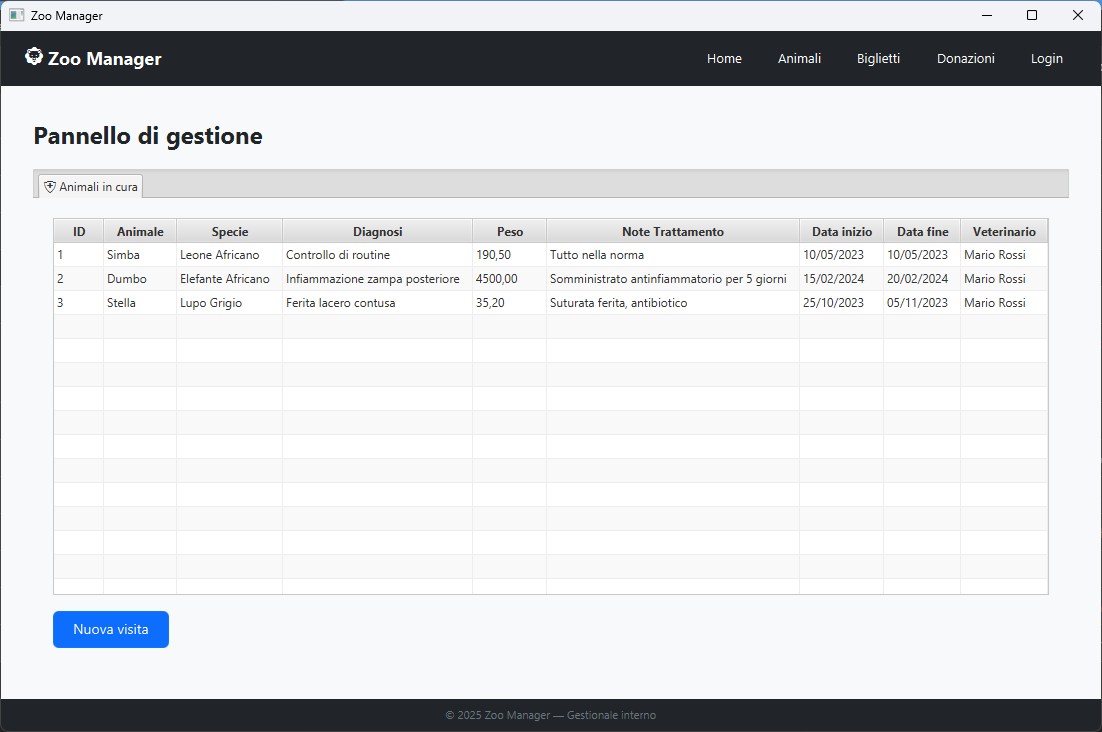
\includegraphics[width=\textwidth]{schermate/LoginVeterinario.png}
    \caption {Immagine della schermata di loged come veterinario}

    \label{fig:schermataLogedVeterinario}
\end{figure}


\subsection{Schermata dal punto di modifica di un animale (Admin)}

Questa schermata consente all'amministratore di modificare i dati relativi a un animale presente nel sistema. Attraverso l'apposito modulo è possibile aggiornare informazioni anagrafiche, caratteristiche, habitat e altri dati gestionali associati all'animale selezionato.

\begin{figure}[H]
    \centering
    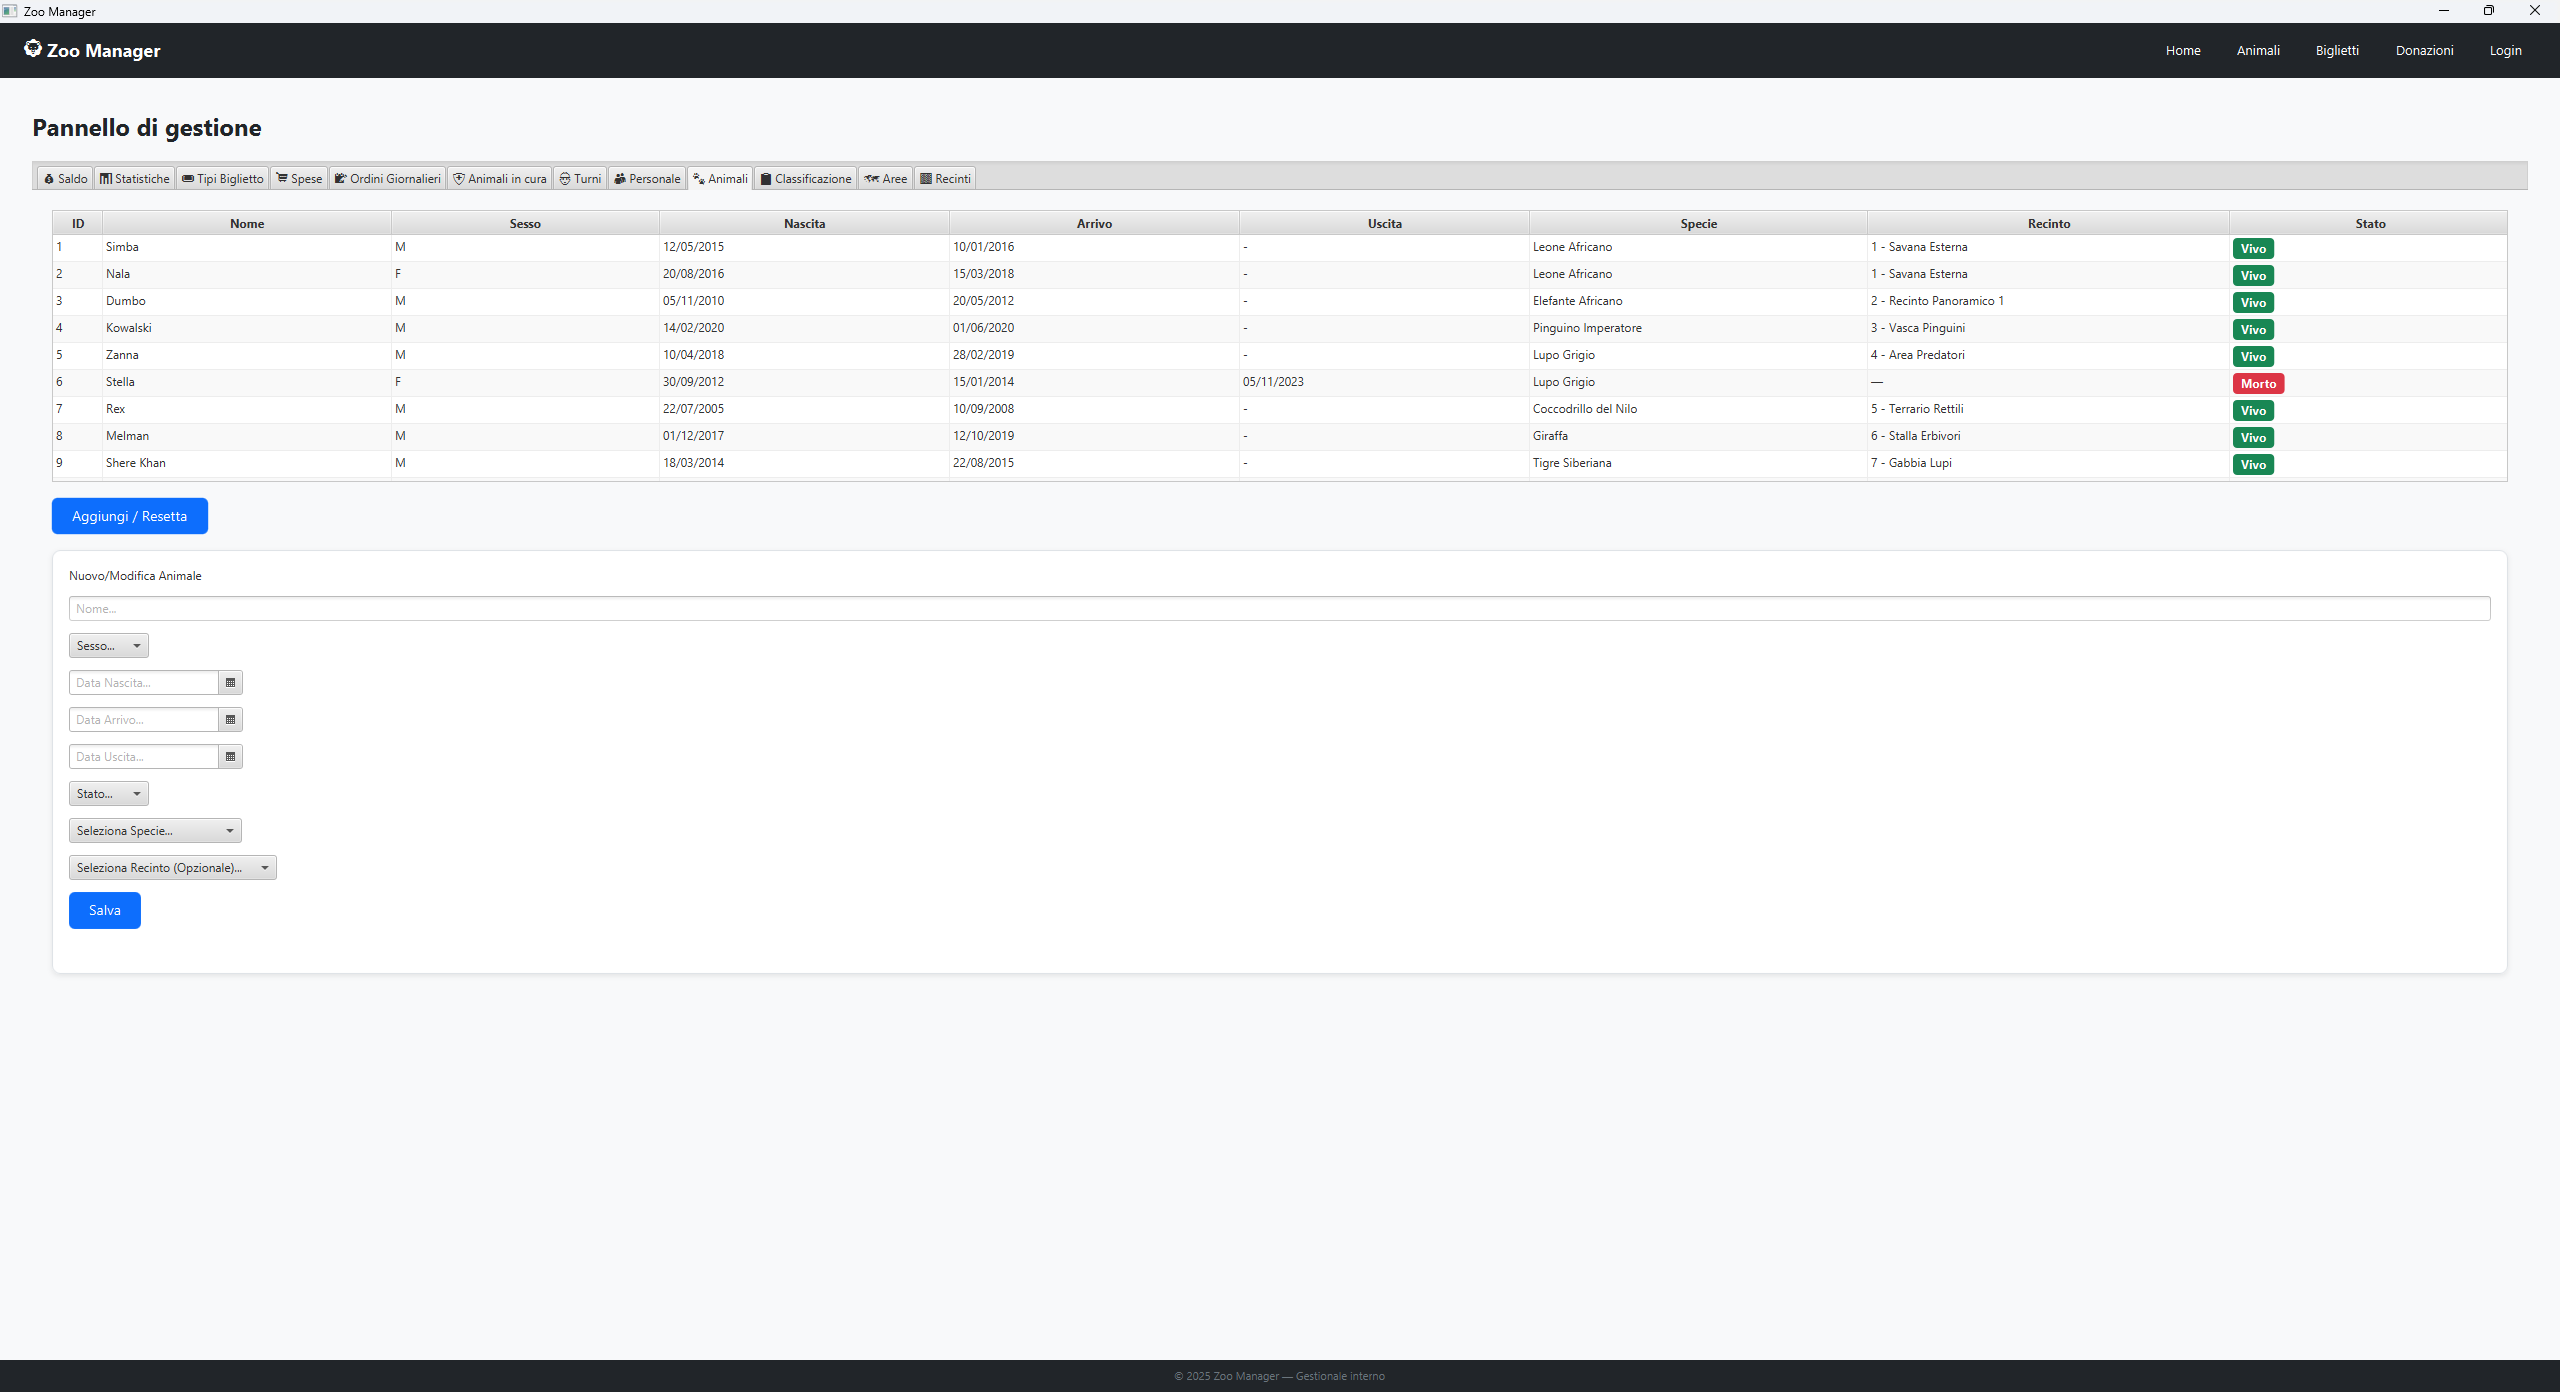
\includegraphics[width=\textwidth]{schermate/adminAnimaliModifiche.png}
    \caption {Immagine della schermata di modifica di un animale loged come Admin}

    \label{fig:schermataanimalimodifiche}
\end{figure}

\end{document}
